\setcounter{tocdepth}{6}
\setcounter{secnumdepth}{6}

\pagenumbering{arabic} % Arabic (standard) page numbering
\clearpage

\begin{abstract}
  The purpose of this project is to create a proof of concept server that receives Linux syscall requests from a client, executes them, and sends back their response.
\\

  This has applications in confidential computing environments where a target program is running in a `sealed' virtual environment, but still needs some access to the host's Linux kernel. 
\\

  The target program's syscalls are intercepted by a client that forwards the syscalls to the server that is running somewhere else, for example on the host machine. The server executes the syscalls and returns their response to the target program, as if the syscall was performed in the target program's environment.

\end{abstract}

\tableofcontents

\chapter{Project Plan}

In order to create a syscall server, there must also be a process and a client that intercepts this process's syscalls and forwards them to the server.

Let's begin by first having a look at the normal execution of a process in a Linux-based operating system: the process communicates directly with the kernel.

\begin{figure}[h]
\centering
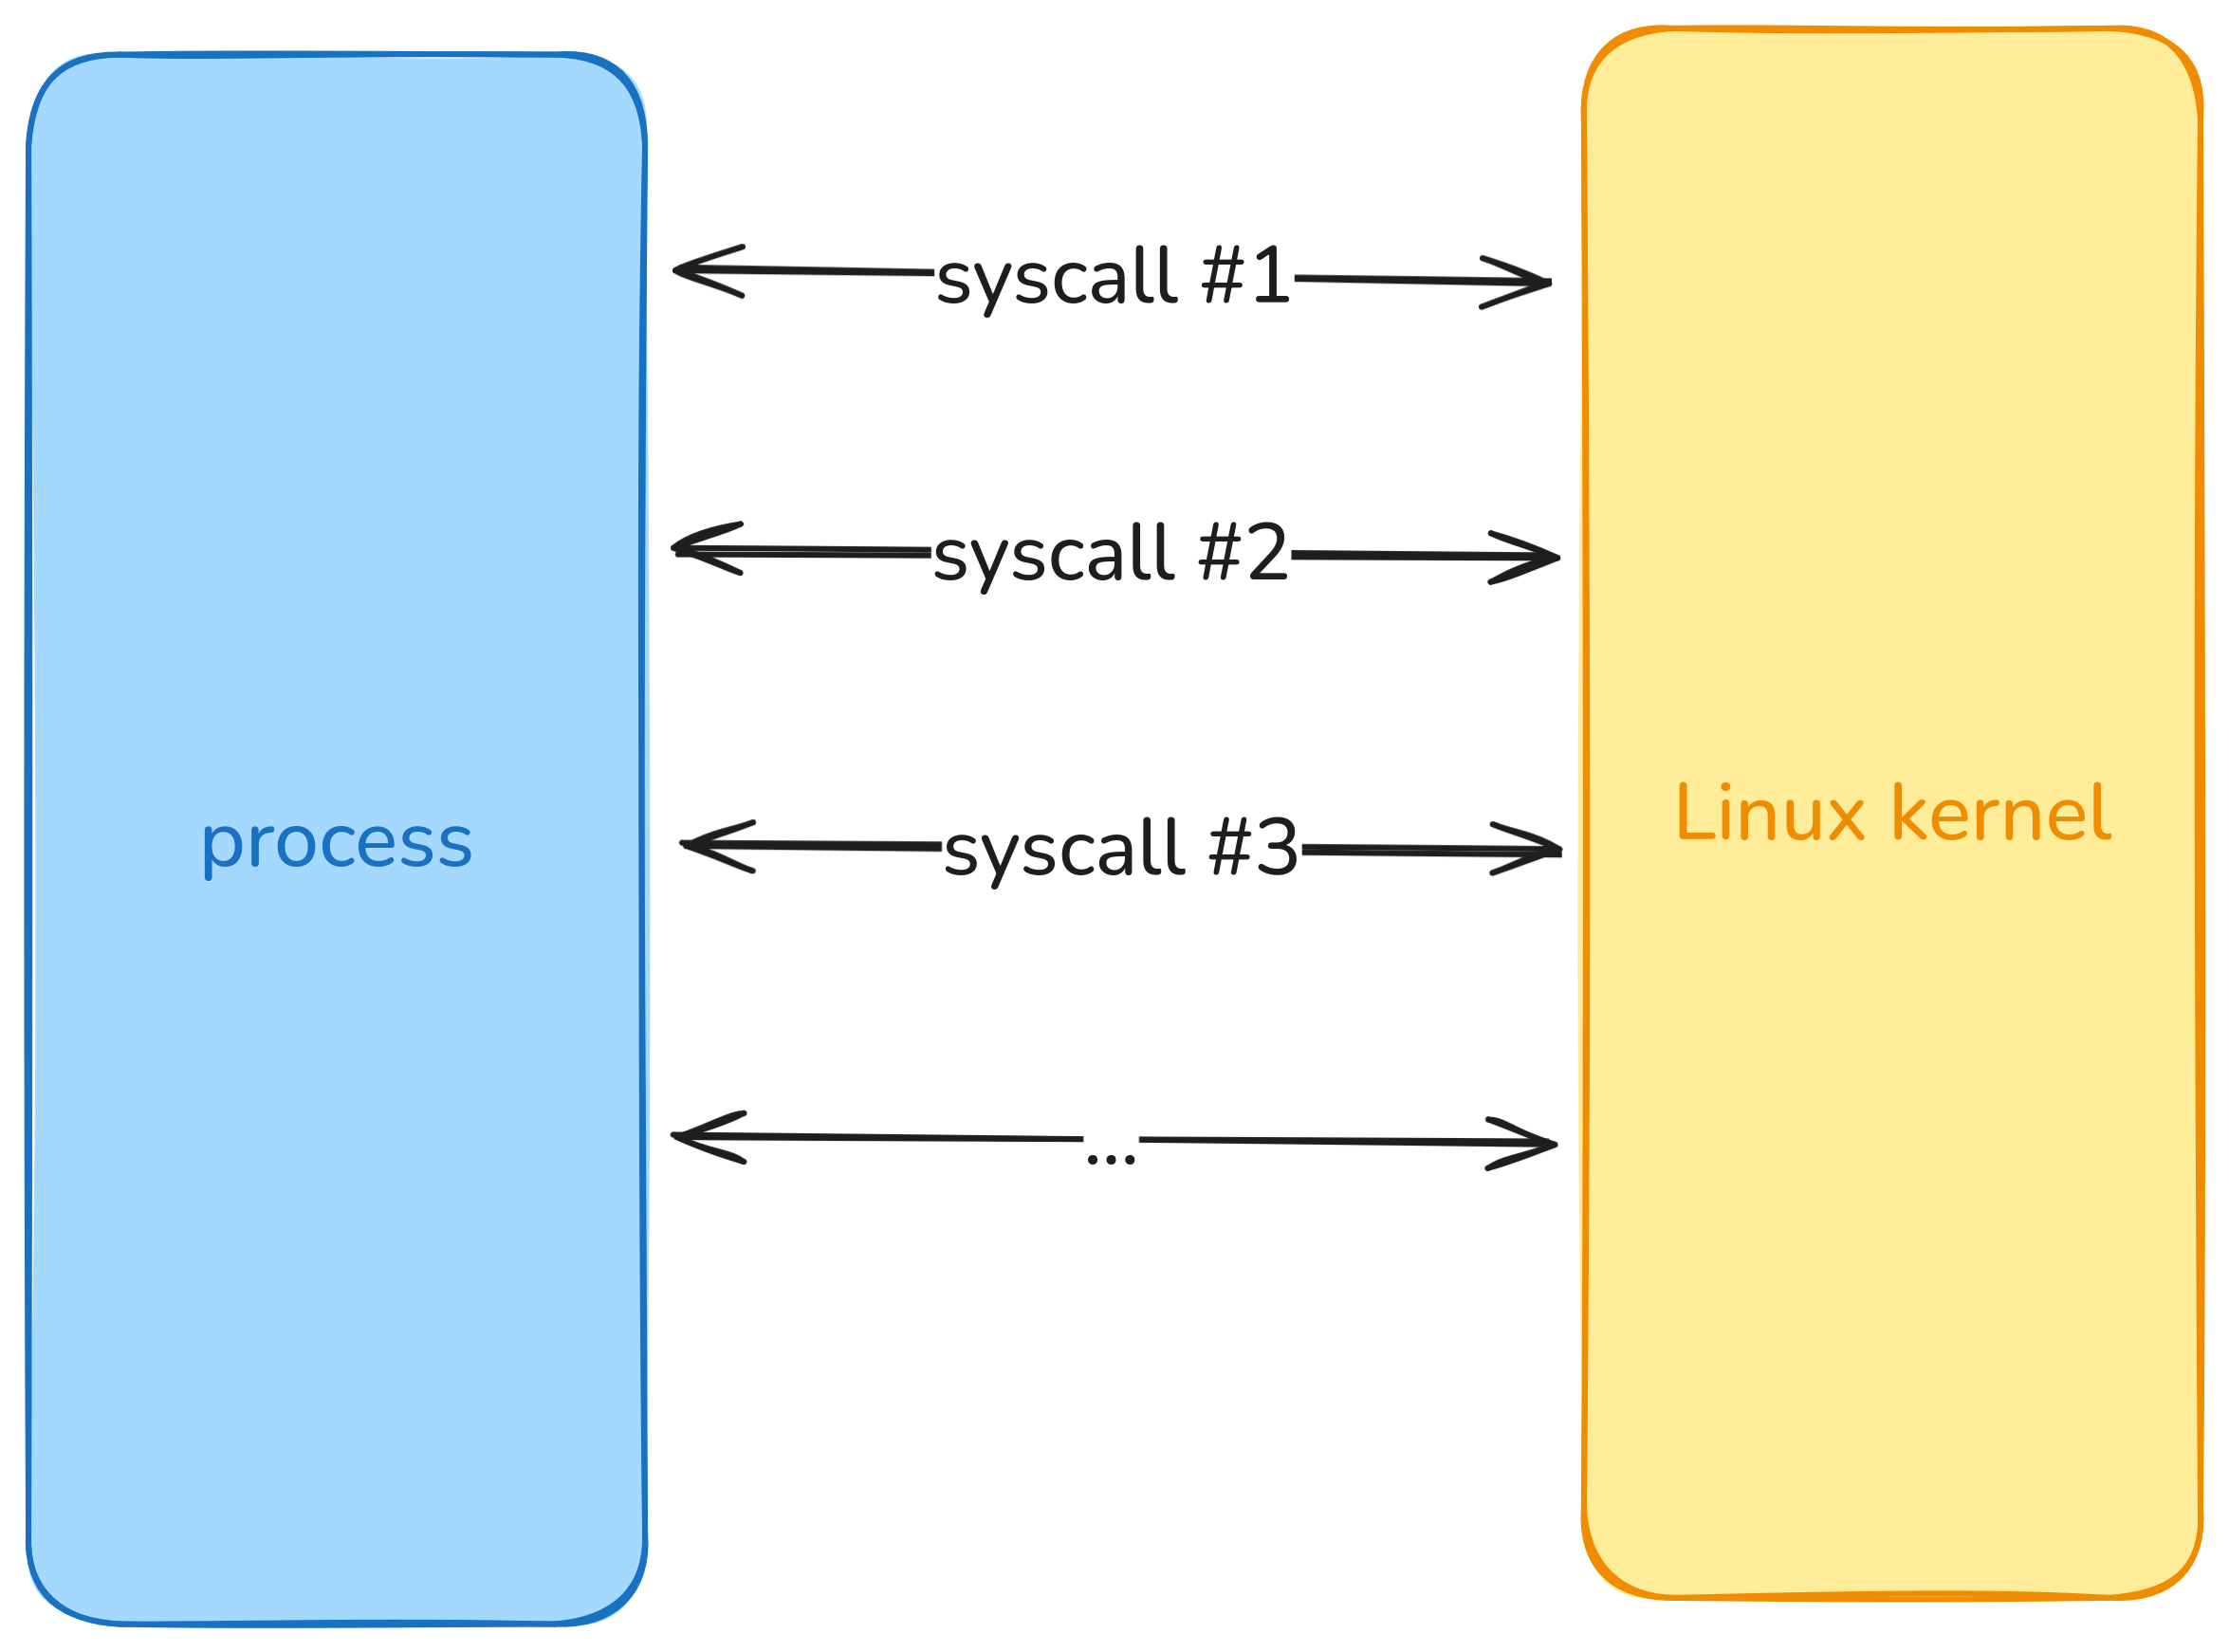
\includegraphics[width=0.4\textwidth]{images/process_syscall_normal.png}
\caption{Direct syscalls to Linux kernel}
\end{figure}

The goal of this project is to create a server capable of receiving and resolving syscall requests as shown in the diagram below.

\begin{figure}[h]
\centering
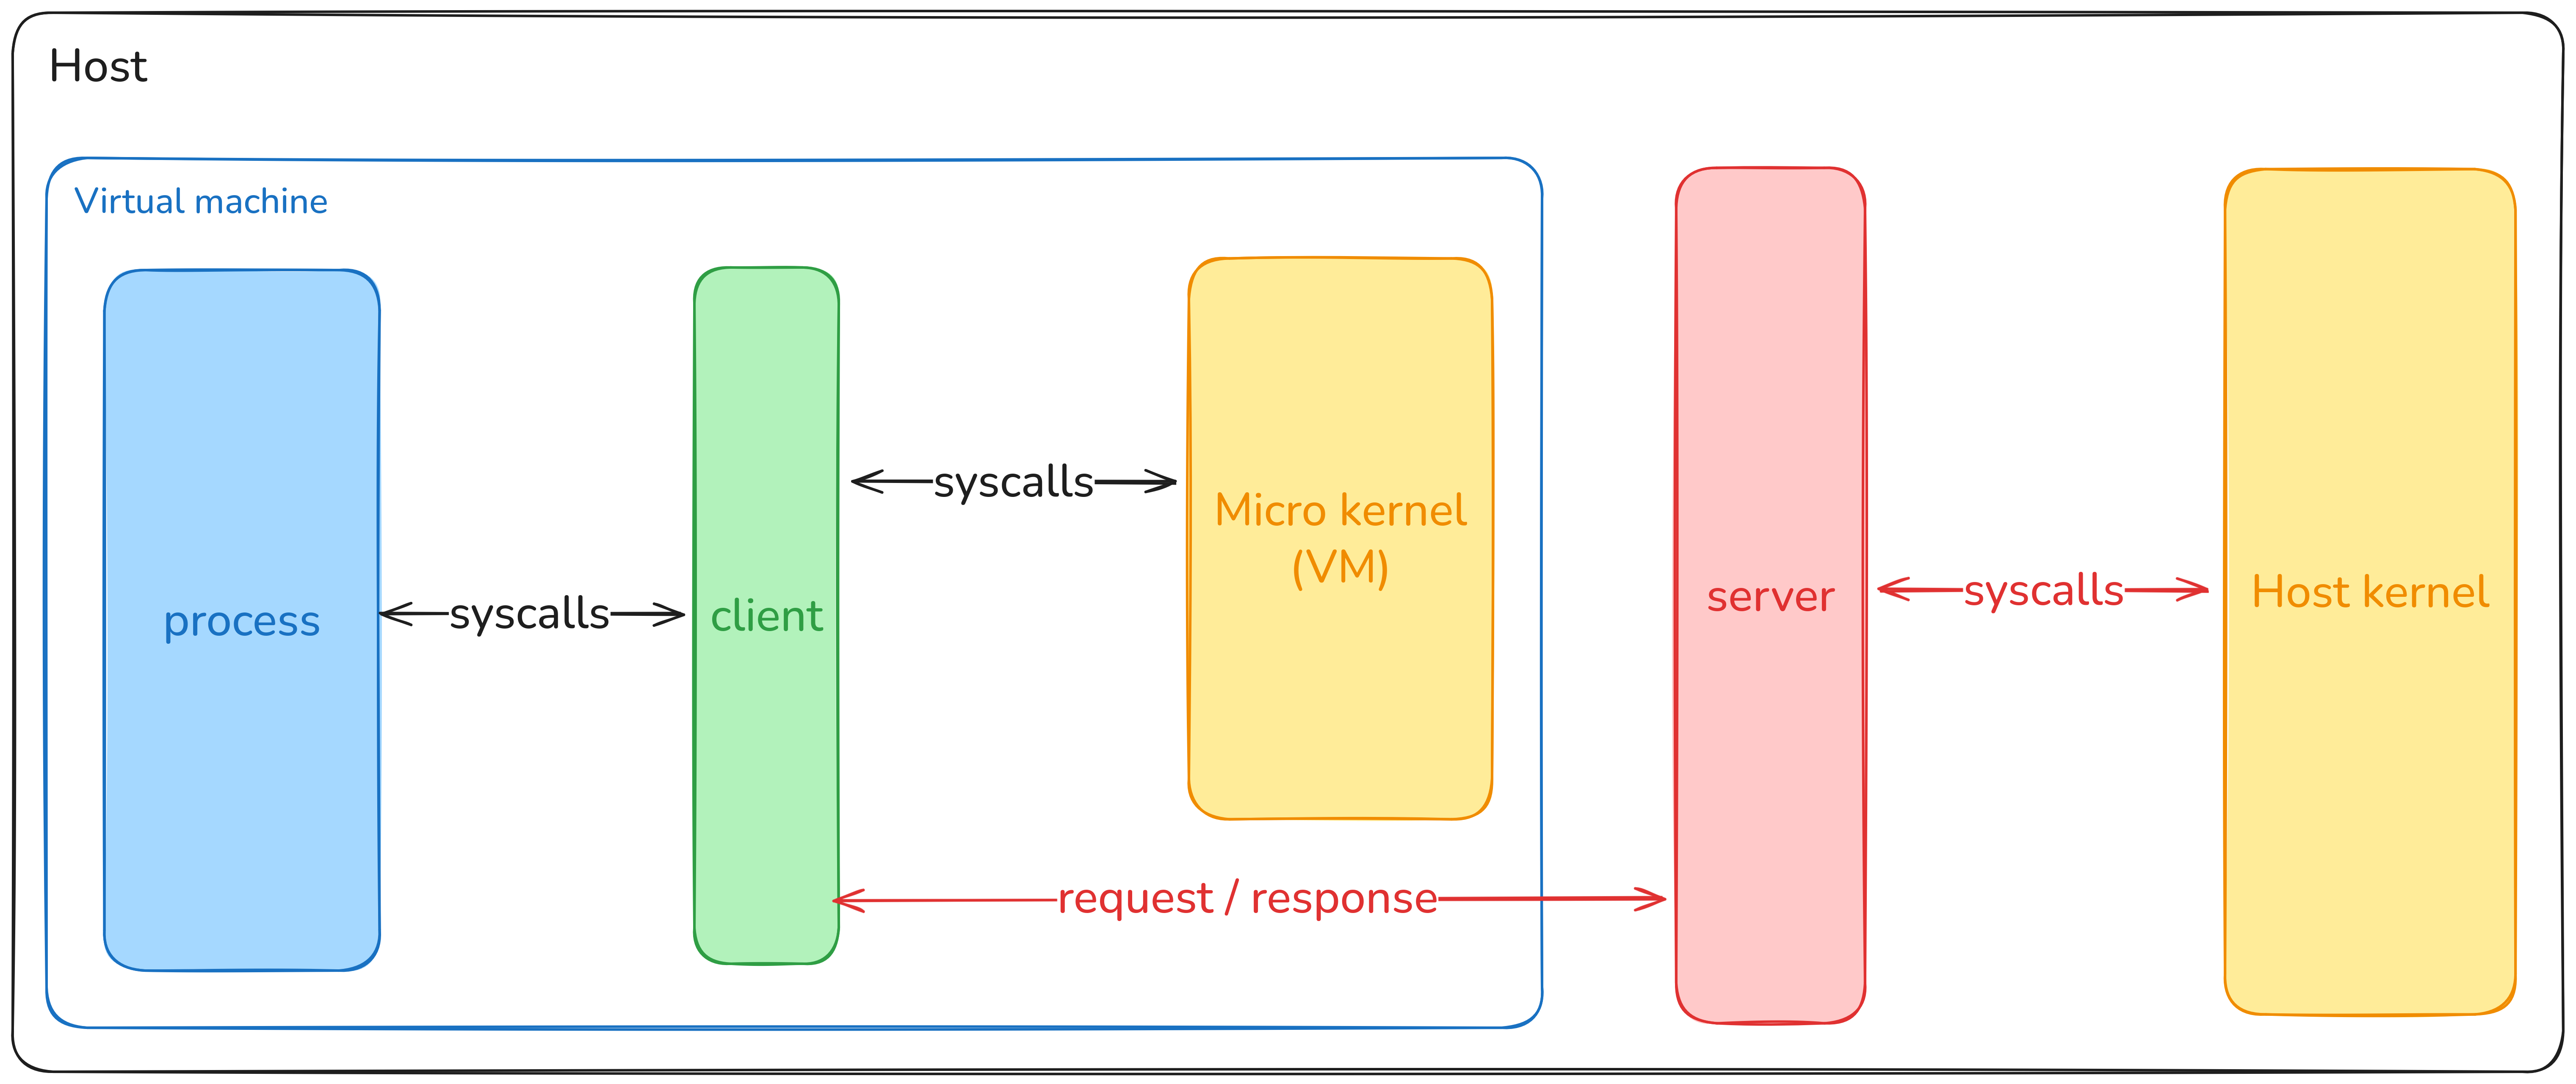
\includegraphics[width=0.95\textwidth]{images/process_syscall_intercept_vm.png}
\caption{Syscall interception and forwarding in a containerized environment}
\end{figure}

Although this project's focus is the server, we also need a target program and client in order to test the server's functionality.

For simplicity's sake, during the development of the server, the target program and client will run directly on the host machine. As shown in the diagram below.

\begin{figure}[h]
\centering
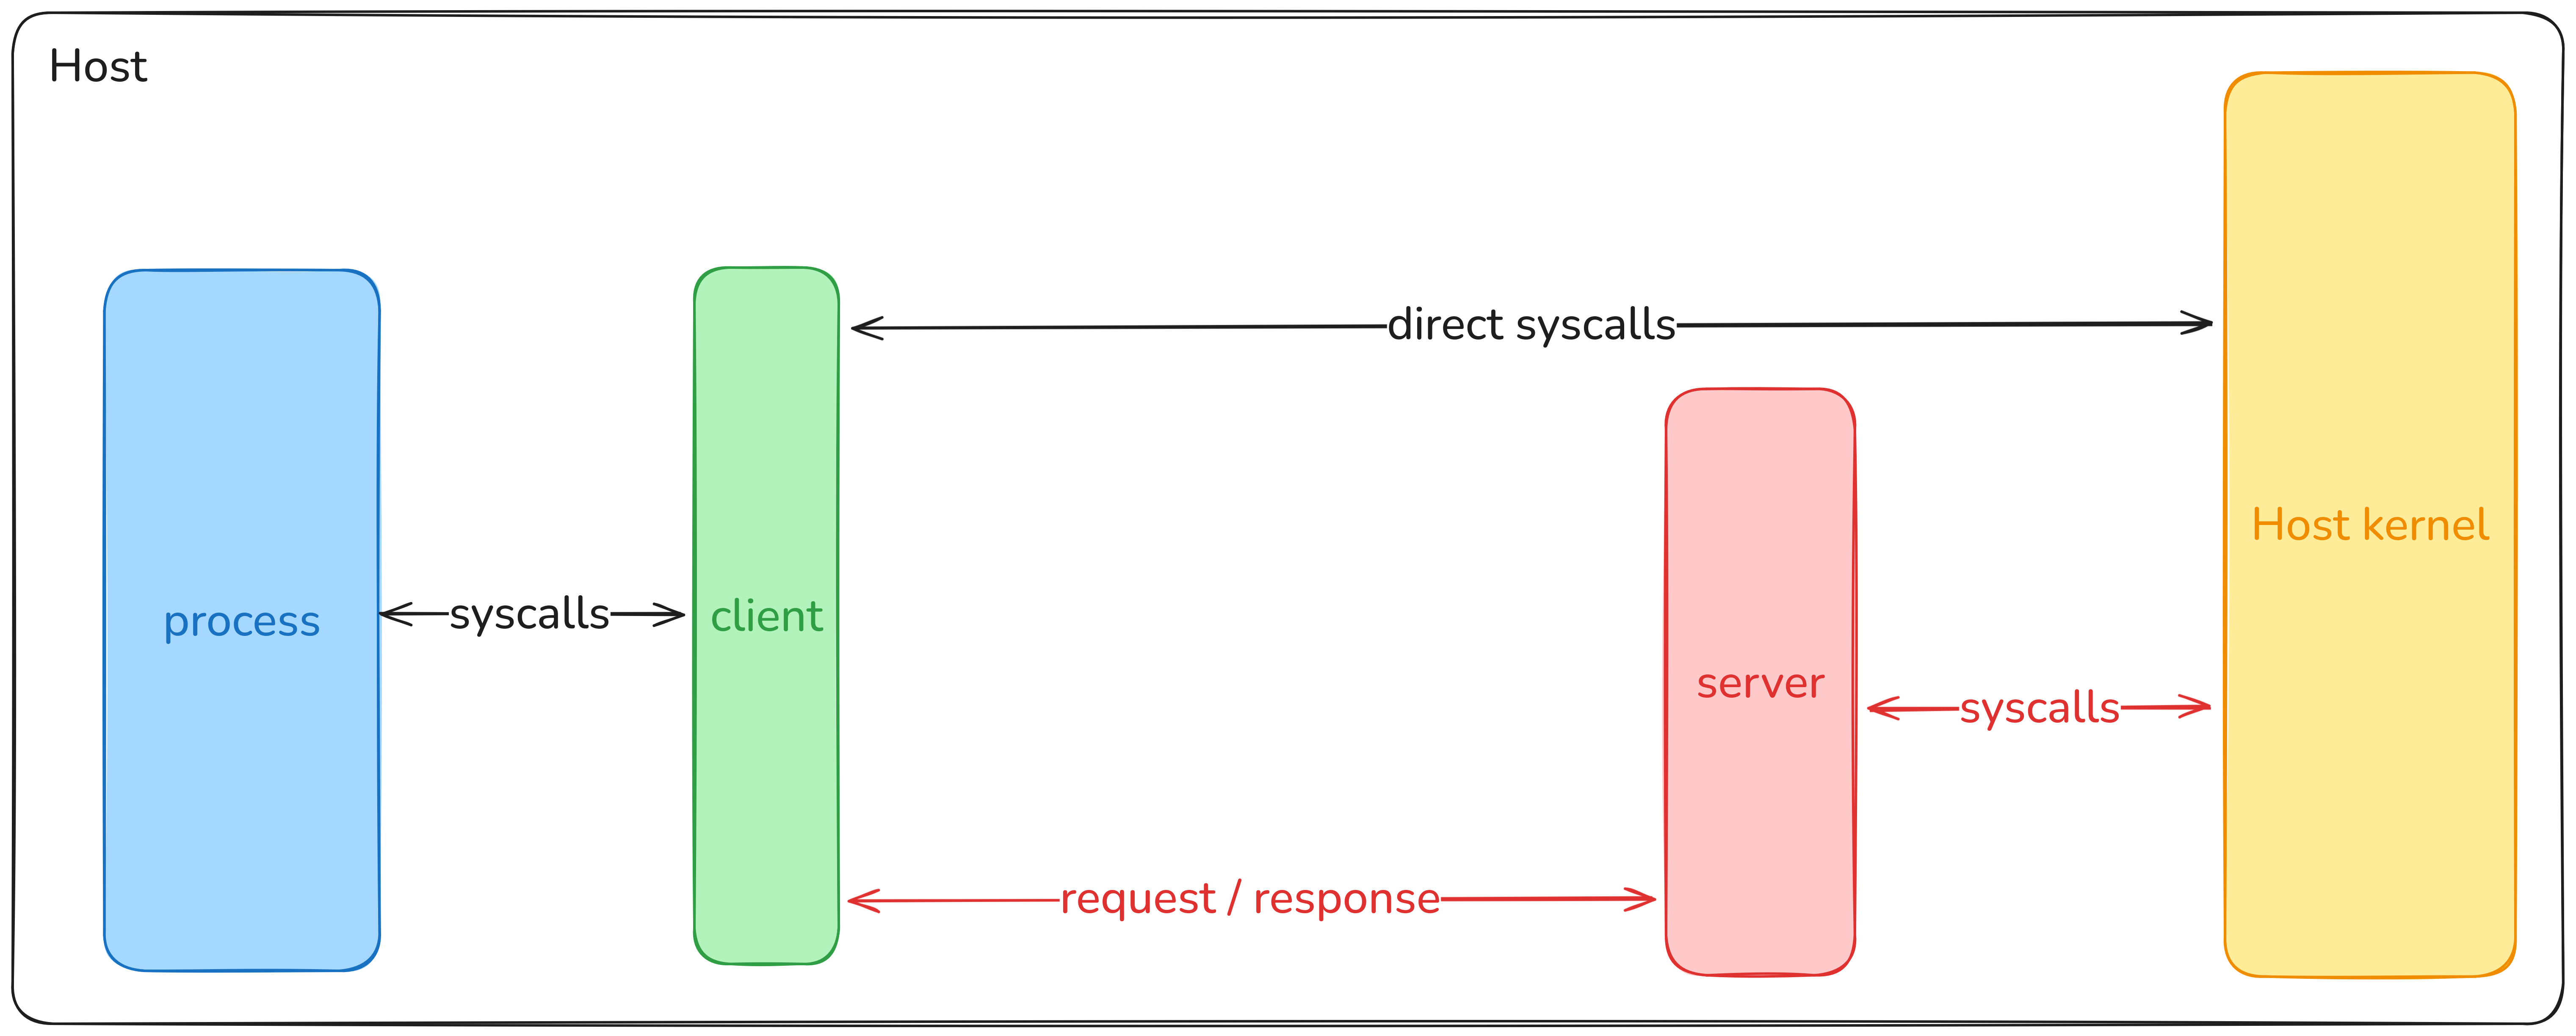
\includegraphics[width=0.95\textwidth]{images/process_syscall_intercept_host.png}
\caption{Syscall interception and forwarding in the context of this project's development}
\end{figure}

As you can see, not all of the syscalls are intercepted by the client. This is because some operations must be run directly by the target process in order to function properly, for example memory allocation.

\chapter{Research}

There are many topics to be research and decisions to be made in order to start this project. In this chapter I will go over them one by one.

\section{Programming language}

Since we are working with Linux system calls, I picked the obvious choice for the programming language to be used in this project: C.

This is because there is a native Linux syscall api for the C programming language, since the kernel itself is written in C.

\section{Syscall interception}

There were two approaches I considered when it comes to system call interception:

\begin{itemize}
  \item Modifying the standard C system library with my own syscall implementations.
  \item Creating a shared library containing custom syscall implementations, and loading it before before all the other shared libraries.
\end{itemize}

I chose the latter, since it's easier to implement and it can be used with any program as long as it's not statically compiled, which is the case for most programs.

\subsection{Which syscalls to implement}

There are hundreds of system calls that the Linux kernel supports. Because of the relatively limited time allocated for this project, I chose to implement some of the most common ones.
\\

The first system calls that came to my mind were file operations like open(), read(), write() and close(). This was a good start, but in order to have a clearer idea of what system calls to implement, I have decided to take an existing program and have a look at what system calls it uses.
\\

The program I chose to analyze is sqlite3, since it's a widely used tool that isn't too complex in terms of what system operations it needs.
\\

I started by using the strace tool, in order to see what system calls are used by sqlite3. I soon found out that sqlite3 heavily relies on one particular system call: mmap(). 

This syscall allows a program to map files to a certain region in memory, so that all changes made to that specific memory region are reflected onto the file.

Since there is no practical way of intercepting direct memory writes, it is impossible to delegate the mmap() syscall to the server. 
\\

Fortunately if you build sqlite3 from source, you can disable the mmap() syscall by using specific compilation flags. After compiling sqlite3 from source with mmap() disabled I was able to get a list of syscalls I could intercept.
\\

This is the list of syscalls I had to implement in order to delegate all of sqlite3's execution to the server.

\begin{multicols}{4}
\begin{itemize}
  \item access()
  \item close()
  \item fnctl()
  \item fdatasync()
  \item fstat()
  \item getcwd()
  \item ioctl()
  \item lseek()
  \item newfstatat()
  \item open()
  \item openat()
  \item pread()
  \item prlimit()
  \item pwrite()
  \item read()
  \item stat()
  \item unlink()
  \item write()
\end{itemize}
\end{multicols}

\section{Client-server communication}

There are many options when it comes to exposing the server API to the client. I've decided to use Unix domain sockets since they allow processes to communicate locally using the filesystem as their address space. 
This comes with the advantage of the possibility to easily switch to a network socket in the future.
\\

The next step was to choose a communication protocol, at first I tried to implement my own protocol but I quickly abandoned the idea. 

I have found a few viable options for the communication protocol: SunRPC + XDR, eRPC and gRPC + Protobuf.
\\

\begin{table}[h]
\centering
\begin{tabularx}{\textwidth}{|l|X|X|X|}
\hline
\textbf{} & \textbf{SunRPC + XDR} & \textbf{eRPC} & \textbf{gRPC + Protobuf} \\
\hline
\textbf{Primary use} & Simple, classic C RPC & Embedded / real-time RPC & Modern service APIs \\
\hline
\textbf{Dependencies} & Low & Very low & High \\
\hline
\textbf{Speed} & Fast, low overhead & Very fast, minimal overhead & Moderate (higher overhead) \\
\hline
\textbf{Transport} & UDP, TCP & Any & HTTP/2 \\
\hline
\textbf{Adoption} & Moderate (legacy, systems) & Niche (embedded) & Very high (cloud, microservices) \\
\hline
\end{tabularx}
\caption{Comparison of RPC frameworks}
\end{table}

They all have their own advantages and disadvantages, I ultimately chose SunRPC + XDR since it's lightweight, fast and widely used.

\section{Server}

The server implementations itself was quite straight forward. The main challenge was understanding how the syscalls work. I will be talking more about this in the chapter about the server implementation.
\\

I've decided that the server will accept only one client connection, to allow me to progress faster on other parts of the project. It would have been nice to have the ability to server multiple clients, but I didn't have time to implement it. Nonetheless the current server architecture was more than enough for the scope of this project.

\section{Notes}

The research phase was heavily assisted by the professor, and also by AI.
\\

This helped expedite the research process by providing a clearer direction on where and what to research.

\chapter{Implementation}

\section{Experimenting and use of AI}

Since this project has many moving parts, the first thing I did was create small toy projects in order to better understand each tool and part of the project.
I have created a few Unix socket client/server programs, and I've also played around with the syscall interception mechanism.
\\

With the information gathered from building the client/server toy programs, I've used AI (Claude Code) to create the project's structure and boilerplate code. The code wasn't perfect, but it was a starting point.
\\

The most value AI has brought to this project were the documentation files I've asked it to generate. I have explicitly asked the AI to create an extensive developer documentation on how all the project's pieces should function together. These documentation files reside in the \textit{\detokenize{docs/dev_docs/}} folder.
\\

This was especially useful for better understanding SunRPC + XDR, since I've found that online documentation is very hard to navigate.

\section{Code structure}

This project contains a lot of folders because I have decided to keep all code and documentation I wrote, as well as the sources for sqlite3. This is the project's directory structure:

\begin{description}

  \item[\texttt{\detokenize{build/}}]
  - build artifacts.

  \item[\texttt{\detokenize{docs/}}]
  - markdown files for notes and documentation.
  \begin{itemize}
    \item \texttt{\detokenize{dev_docs/}} - AI generated developer documentation
    \begin{itemize}
      \item \texttt{\detokenize{00_README.md}}
      \item \texttt{\detokenize{01_INTRODUCTION.md}}
      \item \texttt{\detokenize{02_ARCHITECTURE.md}}
      \item \ldots
    \end{itemize}
    \item \texttt{\detokenize{journal.md}} - developer journal
    \item \texttt{\detokenize{sqlite3_syscalls.md}} - list of syscalls used by sqlite3
    \item \texttt{\detokenize{todo.md}} - tasks
  \end{itemize}

  \item[\texttt{\detokenize{playground/}}]
  - experimental examples.

  \item[\texttt{\detokenize{sqlite-amalgamation-3510100/ and sqlite-src-3510100/}}]
  - sqlite3 source code.

  \item[\texttt{\detokenize{src/}}]
  - project's source code.
  \begin{itemize}
    \item \texttt{\detokenize{intercept/}} - syscall interception headers
    \item \texttt{\detokenize{program.c}} - test program
    \item \texttt{\detokenize{protocol/protocol.x}} - protocol definition
    \item \texttt{\detokenize{rpc_client.c}} - intercept client
    \item \texttt{\detokenize{rpc_server.c}} - syscall server
    \item \texttt{\detokenize{transport_config.h}} - transport layer config
  \end{itemize}

  \item[\texttt{\detokenize{Makefile}}]
  - build scripts.

  \item[\texttt{\detokenize{test_query.sql}}]
  - test SQL query.

\end{description}

\subsection{playground/}

The playground folder contains the tests programs written before starting the full implementation of the project

\subsection{docs/}

This folder contains markdown documents used to keep track of this project's todos, as well as developer documentation in the \textbf{\detokenize{dev_docs/}} subfolder.

The files in the \textbf{\detokenize{dev_docs/}} subfolder were generated by AI in the early stages of this project.

\subsection{src/}

This is the main source code for the project. It contains the client and server code, as well as the communication protocol definition.

\section{Protocol}

Let's start by analyzing the RPC protocol definition, since it's the glue between the client and the server.


The protocol definition lives in the \textit{src/protocol/protocol.x} file.

\begin{lstlisting}[style=mycode, language=C, caption={protocol.x code snippet}]
/* Maximum path length for open() */
const MAX_PATH_LEN = 4096;

/* Maximum buffer size for read/write operations */
const MAX_BUFFER_SIZE = 1048576;  /* 1MB */

// Syscall request/response structures
struct open_request {
    string path<MAX_PATH_LEN>;  /* File path */
    int flags;                   /* Open flags (O_RDONLY, O_WRONLY, etc.) */
    unsigned int mode;           /* Permission mode */
};

struct open_response {
    int fd;          /* File descriptor (client-side mapped FD) */
    int result;      /* Return value: fd on success, -1 on error */
    int err;         /* errno value */
};

// ...

// RPC Program Definition
program SYSCALL_PROG {
    version SYSCALL_VERS {
        open_response SYSCALL_OPEN(open_request) = 1;
        openat_response SYSCALL_OPENAT(openat_request) = 2;

        // ...

    } = 1;  /* Version 1 */
} = 0x20000001;  /* Program number */
\end{lstlisting}

There are 3 main sections in the \textit{protocol.x} file.
\begin{itemize}
  \item \textbf{const declarations} - used as configuration variables
  \item \textbf{syscall request/response structs} - they define the data structures used for the client/server communication
  \item \textbf{RPC program definition} - defines the API exposed by the server by using the previously defined structs. 
\end{itemize}

This file provides an abstract definition of our protocol. In order to make requests and receive responses to/from the server, we need access to the protocol's C implementation.
\\

To generate the protocol's implementation we can run the following command:
\begin{commandline}
\begin{verbatim}
$ make rpc_gen

cd ./src/protocol/ && rpcgen -C protocol.x
\end{verbatim}
\end{commandline}

This command generates 4 additional files in the \textit{src/protocol/} folder:
\begin{itemize}
  \item \textbf{\detokenize{protocol_clnt.c}} - protocol client API.
  \item \textbf{\detokenize{protocol_svc.c}} - protocol server API.
  \item \textbf{\detokenize{protocol_xdr.c}} - serialization/deserialization logic.
  \item \textbf{protocol.h} - bundles request/response data structures, protocol configuration and client/server APIs.
\end{itemize}

\section{Client}

The client is implemented by the \textit{\detokenize{src/rpc_client.c}} file, while the system call override functions are located in the \textit{\detokenize{src/intercept/}} folder.

To compile the client you can use the following command:
\begin{commandline}
\begin{verbatim}
$ make client 

gcc -Wall -g -I/usr/include/tirpc -I./src/protocol/ -I./src/
-shared -fPIC -o ./build/intercept.so \textbackslash ./src/rpc_client.c
\textbackslash ./src/protocol/protocol_xdr.c \textbackslash .
/src/protocol/protocol_clnt.c \textbackslash -ltirpc -ldl
\end{verbatim}
\end{commandline}


The client is compiled as a shared library located in \textit{\detokenize{build/intercept.so}}, and it has 2 main functions:

\begin{itemize}
  \item Establish connection to the server
  \item Intercept syscalls and forward them to the server
\end{itemize}

In order to use the client you must load the compiled shared library before all other shared libraries, by setting the \textit{\detokenize{LD_PRELOAD=build/intercept.so}} environment variable.
\\

Since our client shared library is loaded before all other libraries, including \textit{libc} which contains the usual implementations of the system calls; we can override and, thus intercept, syscalls.
\\

This is a simplified example of a syscall override:

\begin{lstlisting}[style=mycode, language=C, caption={simplified syscall override example}]
  // Identical syscall signature as the one in 'libc'
  int open(const char *pathname, int flags, ...) {
    
    CLIENT *client = get_rpc_client(); /* Get RPC client */
    int result = -1;

    if (client != NULL) {
        /* Prepare RPC request */
        open_request req;
        req.path = (char *)pathname; req.flags = flags; req.mode = mode;

        /* Call RPC service */
        open_response *res = syscall_open_1(&req, client);

        if (res != NULL) {
            /* RPC call succeeded */
            result = res->result;
            errno = res->err;
        } else {
            /* RPC call failed */
        }
    } else {
        /* No RPC connection - fall back to direct syscall */
    }

    return result;
}
\end{lstlisting}

This is a simplified example, in the actual syscall implementation there are guards in place to prevent an interception loop, in the eventuality that a syscall interception function calls itself. Below you have a the complete decision tree that illustrates how the syscall interception works.

\clearpage
\thispagestyle{empty}

\vspace*{\fill}
\begin{center}
  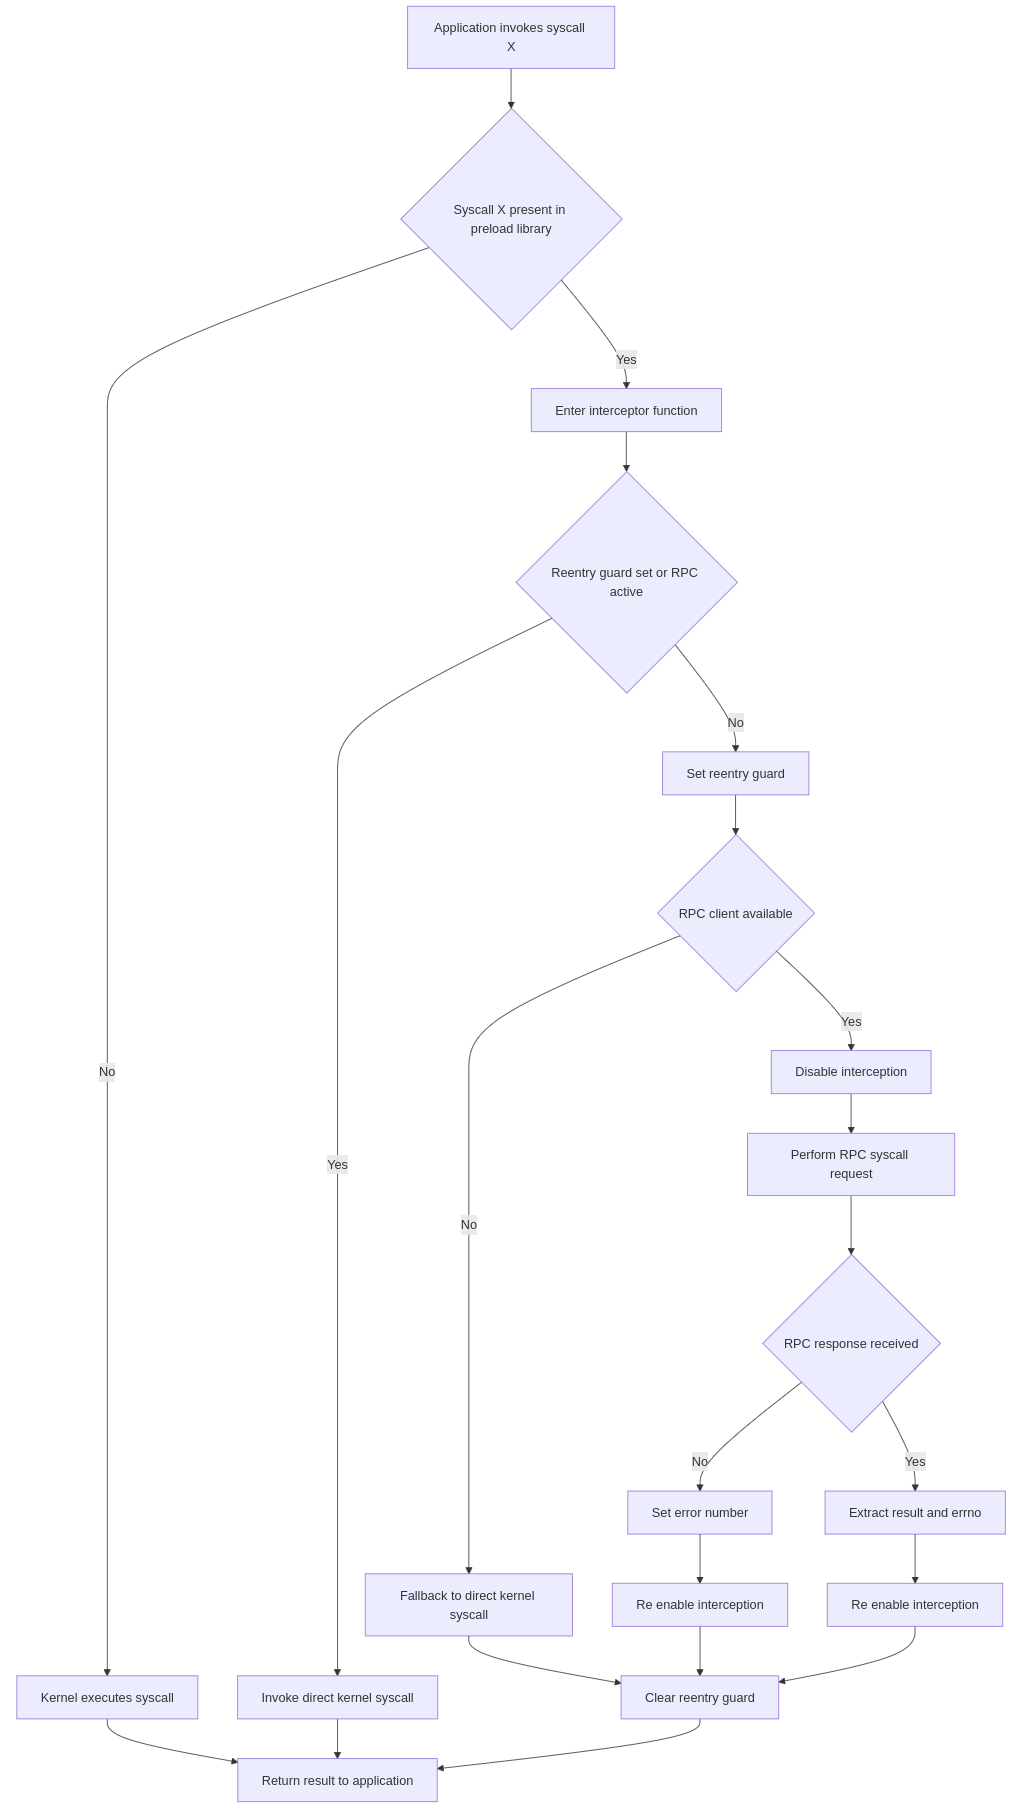
\includegraphics[
    height=0.9\textheight,
    keepaspectratio
  ]{images/client_decision_graph.png}

  \captionof{figure}{Syscall interception decision tree}
\end{center}
\vspace*{\fill}


\section{Server}

All the server's code is located in the \textit{\detokenize{src/rpc_server.c}} file and. In hindsight, it would have been a good idea to separate its logic into multiple files, like the client.
\\

The server's responsibilities are:
\begin{itemize}
  \item Listen for incoming connections
  \item Resolve remote syscall requests
\end{itemize}

For most syscalls, the server just executes them and returns their result to the client. 
\\

But for some syscalls there needs to be some extra logic in order to make them work. This is the case for all system calls that use file descriptors.

\subsection{File descriptor mapping}

Since file descriptors are assigned per process, the server receives the syscalls with the client file descriptors.

In order for the server to be able to use those file descriptors across syscalls, there is a mapping table put in place, that maps the client's file descriptor number to the server's file descriptor.
\\

Below there's an example for an \textit{open()}, \textit{write()} and \textit{close()} syscalls.
\begin{figure}[h]
\centering
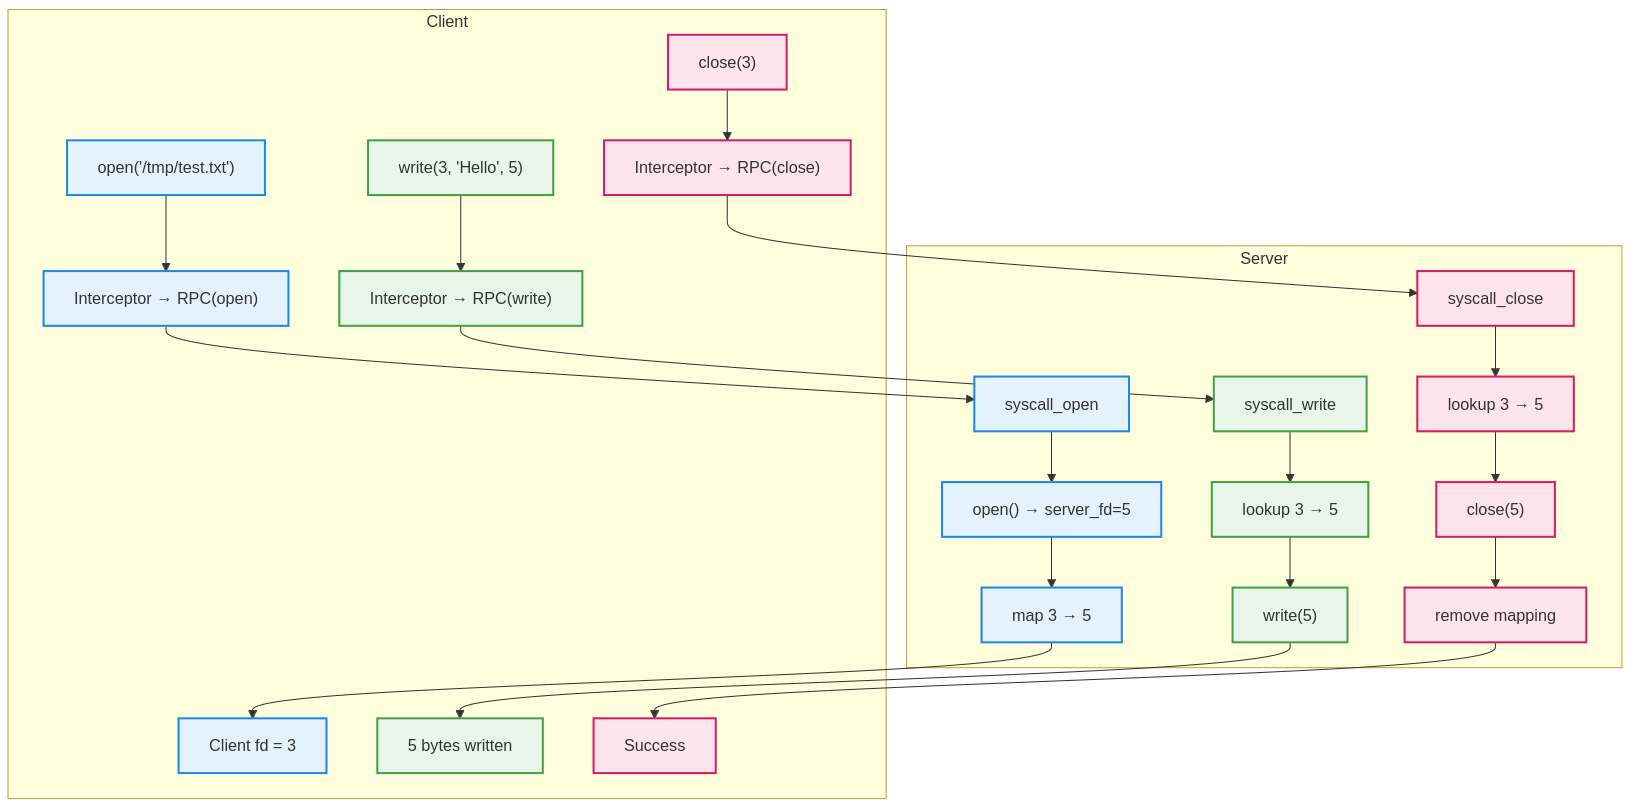
\includegraphics[width=1.0\textwidth]{images/file_descriptor_mapping.png}
\caption{File descriptor mapping flow}
\end{figure}

The file descriptor mapping is done via an array called \textit{\detokenize{fd_mapping}}, and some functions that add, fetch and remove file descriptor mappings.
Client file descriptors are used as indexes for the array.

\begin{landscape}

\section{How it all fits together}

\begin{figure}[H]
    \centering
    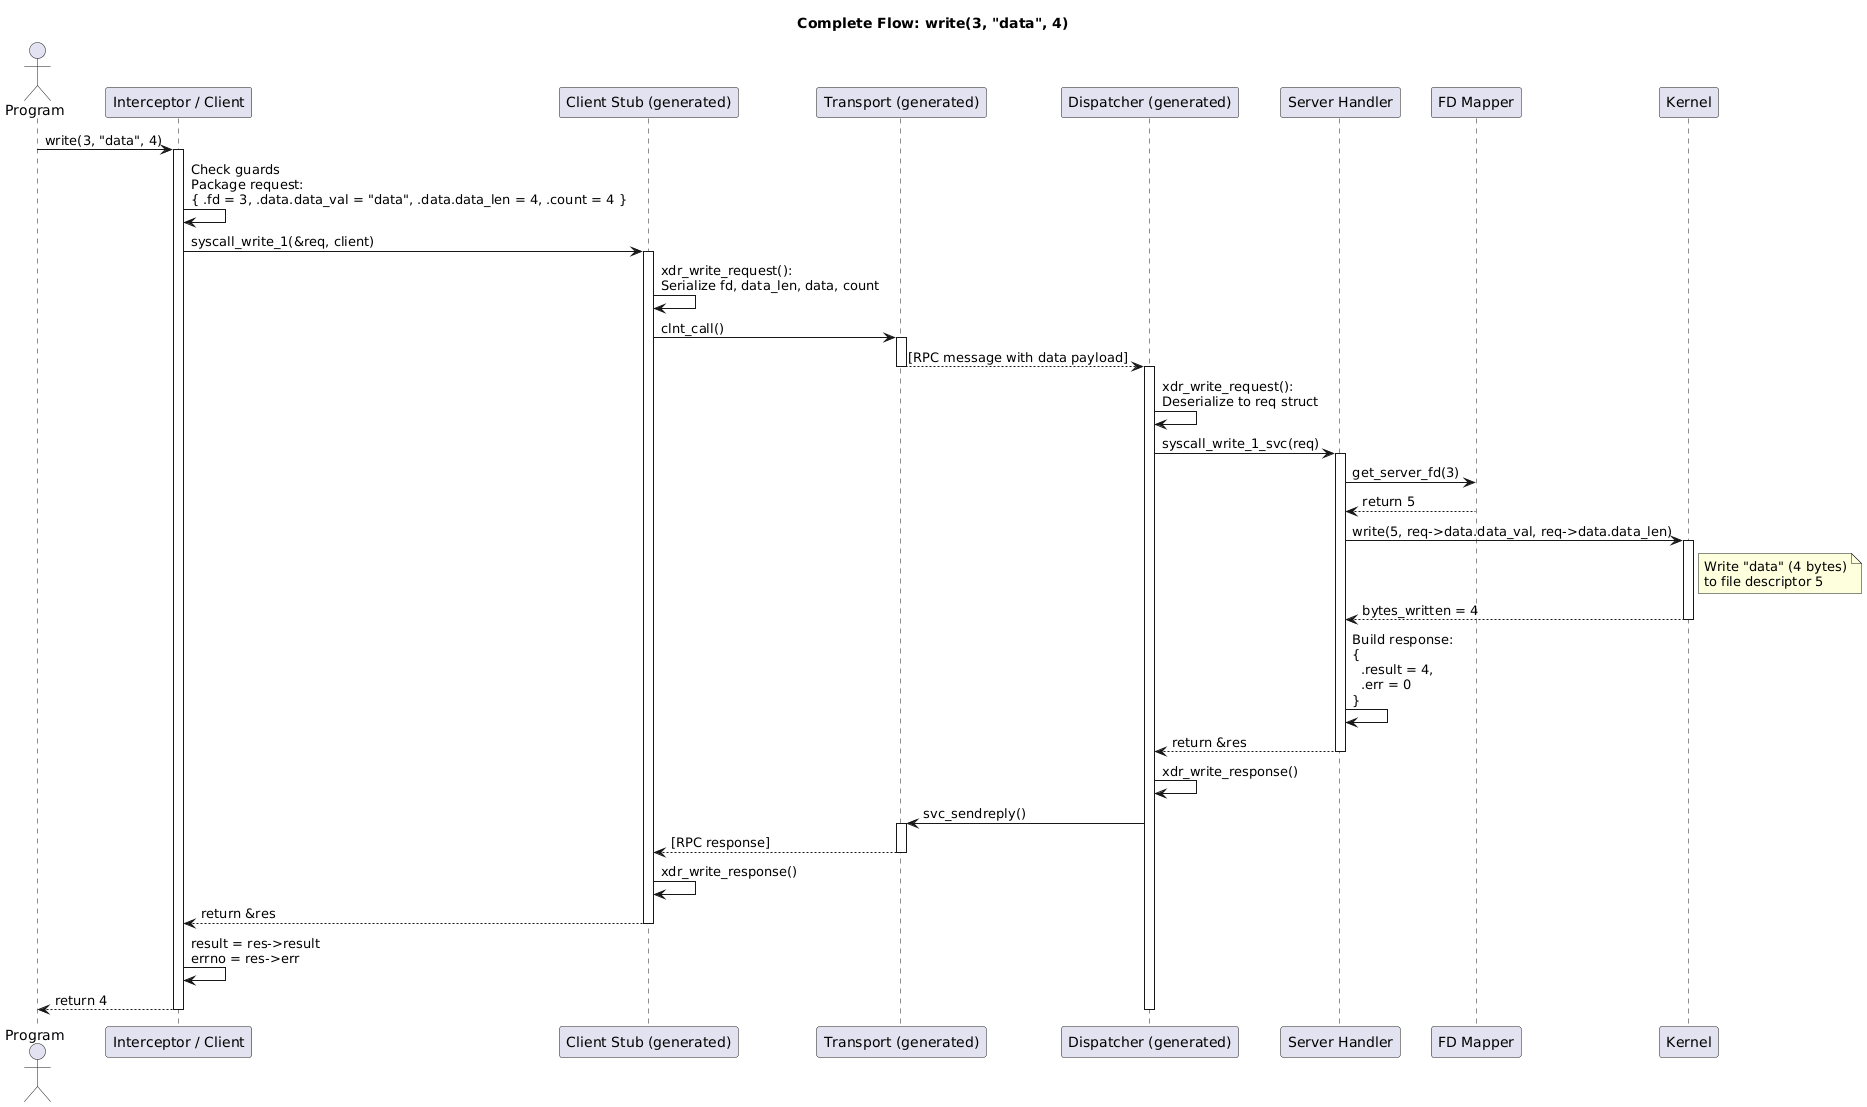
\includegraphics[width=\linewidth]{images/complete_app_flow.png}
    \caption{Complete app flow}
\end{figure}

\end{landscape}

\section{What syscalls have been implemented}

All the syscalls mentioned in the Research chapter have been implemented.

\begin{multicols}{4}
\begin{itemize}
  \item access()
  \item close()
  \item fnctl()
  \item fdatasync()
  \item fstat()
  \item getcwd()
  \item ioctl()
  \item lseek()
  \item newfstatat()
  \item open()
  \item openat()
  \item pread()
  \item prlimit()
  \item pwrite()
  \item read()
  \item stat()
  \item unlink()
  \item write()
\end{itemize}
\end{multicols}

To get to this list I have ran the \textit{strace} command.

\begin{commandline}
\begin{verbatim}
$ make strace -o syscall_list.txt ./sqlite3 testdb.db
\end{verbatim}
\end{commandline}

And within the sqlite3 CLI, I have run the following SQL queries:
\begin{lstlisting}[style=mycode, language=sql, caption={\detokenize{test_query.sql}}]

  CREATE TABLE users (id INTEGER PRIMARY KEY AUTOINCREMENT, name TEXT NOT NULL, email TEXT UNIQUE NOT NULL); 
  
  CREATE TABLE orders (id INTEGER PRIMARY KEY AUTOINCREMENT, user_id INTEGER NOT NULL, product TEXT NOT NULL, amount REAL NOT NULL, FOREIGN KEY (user_id) REFERENCES users(id)); 
  
  INSERT INTO users (name, email) VALUES ('Alice', 'alice@example.com'), ('Bob', 'bob@example.com'); 
  
  INSERT INTO orders (user_id, product, amount) VALUES (1, 'Laptop', 1299.99), (1, 'Mouse', 25.50), (2, 'Keyboard', 75.00);

\end{lstlisting}

Afterwards, I've used \href{https://cyberchef.org/}{cyberchef.org} to get a syscall list alongside their count. You can see the full strace output and the syscall list \href{https://cyberchef.org/#recipe=Regular_expression('User%20defined','%5E(%5BA-z%5D%7C%5B0-9%5D)%2B%5C%5C(',true,true,false,false,false,false,'List%20matches')Unique('Line%20feed',true)Sort('Line%20feed',true,'Numeric')&input=ZXhlY3ZlKCIuL3NxbGl0ZTMiLCBbIi4vc3FsaXRlMyIsICJ0ZXN0ZGIuZGIiXSwgMHg3ZmZlM2QzN2QzZTggLyogNzMgdmFycyAqLykgPSAwCmJyayhOVUxMKSAgICAgICAgICAgICAgICAgICAgICAgICAgICAgICA9IDB4NTVlNGE5MWI3MDAwCm1tYXAoTlVMTCwgODE5MiwgUFJPVF9SRUFEfFBST1RfV1JJVEUsIE1BUF9QUklWQVRFfE1BUF9BTk9OWU1PVVMsIC0xLCAwKSA9IDB4N2YwZDA1ZGE1MDAwCmFjY2VzcygiL2V0Yy9sZC5zby5wcmVsb2FkIiwgUl9PSykgICAgICA9IC0xIEVOT0VOVCAoTm8gc3VjaCBmaWxlIG9yIGRpcmVjdG9yeSkKb3BlbmF0KEFUX0ZEQ1dELCAiL2V0Yy9sZC5zby5jYWNoZSIsIE9fUkRPTkxZfE9fQ0xPRVhFQykgPSAzCmZzdGF0KDMsIHtzdF9tb2RlPVNfSUZSRUd8MDY0NCwgc3Rfc2l6ZT0xMTcxMjcsIC4uLn0pID0gMAptbWFwKE5VTEwsIDExNzEyNywgUFJPVF9SRUFELCBNQVBfUFJJVkFURSwgMywgMCkgPSAweDdmMGQwNWQ4ODAwMApjbG9zZSgzKSAgICAgICAgICAgICAgICAgICAgICAgICAgICAgICAgPSAwCm9wZW5hdChBVF9GRENXRCwgIi9saWIveDg2XzY0LWxpbnV4LWdudS9saWJ6LnNvLjEiLCBPX1JET05MWXxPX0NMT0VYRUMpID0gMwpyZWFkKDMsICJcMTc3RUxGXDJcMVwxXDBcMFwwXDBcMFwwXDBcMFwwXDNcMD5cMFwxXDBcMFwwXDBcMFwwXDBcMFwwXDBcMCIuLi4sIDgzMikgPSA4MzIKZnN0YXQoMywge3N0X21vZGU9U19JRlJFR3wwNjQ0LCBzdF9zaXplPTEyNTM3NiwgLi4ufSkgPSAwCm1tYXAoTlVMTCwgMTI3Mzc2LCBQUk9UX1JFQUQsIE1BUF9QUklWQVRFfE1BUF9ERU5ZV1JJVEUsIDMsIDApID0gMHg3ZjBkMDVkNjgwMDAKbW1hcCgweDdmMGQwNWQ2YjAwMCwgODE5MjAsIFBST1RfUkVBRHxQUk9UX0VYRUMsIE1BUF9QUklWQVRFfE1BUF9GSVhFRHxNQVBfREVOWVdSSVRFLCAzLCAweDMwMDApID0gMHg3ZjBkMDVkNmIwMDAKbW1hcCgweDdmMGQwNWQ3ZjAwMCwgMjg2NzIsIFBST1RfUkVBRCwgTUFQX1BSSVZBVEV8TUFQX0ZJWEVEfE1BUF9ERU5ZV1JJVEUsIDMsIDB4MTcwMDApID0gMHg3ZjBkMDVkN2YwMDAKbW1hcCgweDdmMGQwNWQ4NjAwMCwgODE5MiwgUFJPVF9SRUFEfFBST1RfV1JJVEUsIE1BUF9QUklWQVRFfE1BUF9GSVhFRHxNQVBfREVOWVdSSVRFLCAzLCAweDFkMDAwKSA9IDB4N2YwZDA1ZDg2MDAwCmNsb3NlKDMpICAgICAgICAgICAgICAgICAgICAgICAgICAgICAgICA9IDAKb3BlbmF0KEFUX0ZEQ1dELCAiL2xpYi94ODZfNjQtbGludXgtZ251L2xpYmMuc28uNiIsIE9fUkRPTkxZfE9fQ0xPRVhFQykgPSAzCnJlYWQoMywgIlwxNzdFTEZcMlwxXDFcM1wwXDBcMFwwXDBcMFwwXDBcM1wwPlwwXDFcMFwwXDBwXDIzNlwyXDBcMFwwXDBcMCIuLi4sIDgzMikgPSA4MzIKcHJlYWQ2NCgzLCAiXDZcMFwwXDBcNFwwXDBcMEBcMFwwXDBcMFwwXDBcMEBcMFwwXDBcMFwwXDBcMEBcMFwwXDBcMFwwXDBcMCIuLi4sIDg0MCwgNjQpID0gODQwCmZzdGF0KDMsIHtzdF9tb2RlPVNfSUZSRUd8MDc1NSwgc3Rfc2l6ZT0yMDAzNDA4LCAuLi59KSA9IDAKcHJlYWQ2NCgzLCAiXDZcMFwwXDBcNFwwXDBcMEBcMFwwXDBcMFwwXDBcMEBcMFwwXDBcMFwwXDBcMEBcMFwwXDBcMFwwXDBcMCIuLi4sIDg0MCwgNjQpID0gODQwCm1tYXAoTlVMTCwgMjA1NTgwMCwgUFJPVF9SRUFELCBNQVBfUFJJVkFURXxNQVBfREVOWVdSSVRFLCAzLCAwKSA9IDB4N2YwZDA1YjcyMDAwCm1tYXAoMHg3ZjBkMDViOWEwMDAsIDE0NjIyNzIsIFBST1RfUkVBRHxQUk9UX0VYRUMsIE1BUF9QUklWQVRFfE1BUF9GSVhFRHxNQVBfREVOWVdSSVRFLCAzLCAweDI4MDAwKSA9IDB4N2YwZDA1YjlhMDAwCm1tYXAoMHg3ZjBkMDVjZmYwMDAsIDM1MjI1NiwgUFJPVF9SRUFELCBNQVBfUFJJVkFURXxNQVBfRklYRUR8TUFQX0RFTllXUklURSwgMywgMHgxOGQwMDApID0gMHg3ZjBkMDVjZmYwMDAKbW1hcCgweDdmMGQwNWQ1NTAwMCwgMjQ1NzYsIFBST1RfUkVBRHxQUk9UX1dSSVRFLCBNQVBfUFJJVkFURXxNQVBfRklYRUR8TUFQX0RFTllXUklURSwgMywgMHgxZTIwMDApID0gMHg3ZjBkMDVkNTUwMDAKbW1hcCgweDdmMGQwNWQ1YjAwMCwgNTI4NTYsIFBST1RfUkVBRHxQUk9UX1dSSVRFLCBNQVBfUFJJVkFURXxNQVBfRklYRUR8TUFQX0FOT05ZTU9VUywgLTEsIDApID0gMHg3ZjBkMDVkNWIwMDAKY2xvc2UoMykgICAgICAgICAgICAgICAgICAgICAgICAgICAgICAgID0gMAptbWFwKE5VTEwsIDEyMjg4LCBQUk9UX1JFQUR8UFJPVF9XUklURSwgTUFQX1BSSVZBVEV8TUFQX0FOT05ZTU9VUywgLTEsIDApID0gMHg3ZjBkMDViNmYwMDAKYXJjaF9wcmN0bChBUkNIX1NFVF9GUywgMHg3ZjBkMDViNmY3NDApID0gMApzZXRfdGlkX2FkZHJlc3MoMHg3ZjBkMDViNmZhMTApICAgICAgICAgPSAzODI4NTAKc2V0X3JvYnVzdF9saXN0KDB4N2YwZDA1YjZmYTIwLCAyNCkgICAgID0gMApyc2VxKDB4N2YwZDA1YjZmNjgwLCAweDIwLCAwLCAweDUzMDUzMDUzKSA9IDAKbXByb3RlY3QoMHg3ZjBkMDVkNTUwMDAsIDE2Mzg0LCBQUk9UX1JFQUQpID0gMAptcHJvdGVjdCgweDdmMGQwNWQ4NjAwMCwgNDA5NiwgUFJPVF9SRUFEKSA9IDAKbXByb3RlY3QoMHg1NWU0ODdlMzMwMDAsIDE2Mzg0LCBQUk9UX1JFQUQpID0gMAptcHJvdGVjdCgweDdmMGQwNWRlMTAwMCwgODE5MiwgUFJPVF9SRUFEKSA9IDAKcHJsaW1pdDY0KDAsIFJMSU1JVF9TVEFDSywgTlVMTCwge3JsaW1fY3VyPTgxOTIqMTAyNCwgcmxpbV9tYXg9UkxJTTY0X0lORklOSVRZfSkgPSAwCm11bm1hcCgweDdmMGQwNWQ4ODAwMCwgMTE3MTI3KSAgICAgICAgICA9IDAKaW9jdGwoMCwgVENHRVRTLCB7Y19pZmxhZz1CUktJTlR8SUNSTkx8SVhPTnxJWEFOWXxJTUFYQkVMfElVVEY4LCBjX29mbGFnPU5MMHxDUjB8VEFCMHxCUzB8VlQwfEZGMHxPUE9TVHxPTkxDUiwgY19jZmxhZz1CMzg0MDB8Q1M4fENSRUFEfEhVUENMLCBjX2xmbGFnPUlTSUd8SUNBTk9OfEVDSE98RUNIT0V8RUNIT0t8SUVYVEVOfEVDSE9DVEx8RUNIT0tFLCAuLi59KSA9IDAKaW9jdGwoMSwgVENHRVRTLCB7Y19pZmxhZz1CUktJTlR8SUNSTkx8SVhPTnxJWEFOWXxJTUFYQkVMfElVVEY4LCBjX29mbGFnPU5MMHxDUjB8VEFCMHxCUzB8VlQwfEZGMHxPUE9TVHxPTkxDUiwgY19jZmxhZz1CMzg0MDB8Q1M4fENSRUFEfEhVUENMLCBjX2xmbGFnPUlTSUd8SUNBTk9OfEVDSE98RUNIT0V8RUNIT0t8SUVYVEVOfEVDSE9DVEx8RUNIT0tFLCAuLi59KSA9IDAKcnRfc2lnYWN0aW9uKFNJR0lOVCwge3NhX2hhbmRsZXI9MHg1NWU0ODdjZWVlNTAsIHNhX21hc2s9W0lOVF0sIHNhX2ZsYWdzPVNBX1JFU1RPUkVSfFNBX1JFU1RBUlQsIHNhX3Jlc3RvcmVyPTB4N2YwZDA1YmIxZGYwfSwge3NhX2hhbmRsZXI9U0lHX0RGTCwgc2FfbWFzaz1bXSwgc2FfZmxhZ3M9MH0sIDgpID0gMApnZXRyYW5kb20oIlx4ODlceGM4XHhjOVx4ZDBceDJjXHg5NVx4ZjFceDYxIiwgOCwgR1JORF9OT05CTE9DSykgPSA4CmJyayhOVUxMKSAgICAgICAgICAgICAgICAgICAgICAgICAgICAgICA9IDB4NTVlNGE5MWI3MDAwCmJyaygweDU1ZTRhOTFkODAwMCkgICAgICAgICAgICAgICAgICAgICA9IDB4NTVlNGE5MWQ4MDAwCmFjY2VzcygidGVzdGRiLmRiIiwgRl9PSykgICAgICAgICAgICAgICA9IC0xIEVOT0VOVCAoTm8gc3VjaCBmaWxlIG9yIGRpcmVjdG9yeSkKZ2V0dWlkKCkgICAgICAgICAgICAgICAgICAgICAgICAgICAgICAgID0gMTAwMApzb2NrZXQoQUZfVU5JWCwgU09DS19TVFJFQU18U09DS19DTE9FWEVDfFNPQ0tfTk9OQkxPQ0ssIDApID0gMwpjb25uZWN0KDMsIHtzYV9mYW1pbHk9QUZfVU5JWCwgc3VuX3BhdGg9Ii92YXIvcnVuL25zY2Qvc29ja2V0In0sIDExMCkgPSAtMSBFTk9FTlQgKE5vIHN1Y2ggZmlsZSBvciBkaXJlY3RvcnkpCmNsb3NlKDMpICAgICAgICAgICAgICAgICAgICAgICAgICAgICAgICA9IDAKc29ja2V0KEFGX1VOSVgsIFNPQ0tfU1RSRUFNfFNPQ0tfQ0xPRVhFQ3xTT0NLX05PTkJMT0NLLCAwKSA9IDMKY29ubmVjdCgzLCB7c2FfZmFtaWx5PUFGX1VOSVgsIHN1bl9wYXRoPSIvdmFyL3J1bi9uc2NkL3NvY2tldCJ9LCAxMTApID0gLTEgRU5PRU5UIChObyBzdWNoIGZpbGUgb3IgZGlyZWN0b3J5KQpjbG9zZSgzKSAgICAgICAgICAgICAgICAgICAgICAgICAgICAgICAgPSAwCm5ld2ZzdGF0YXQoQVRfRkRDV0QsICIvZXRjL25zc3dpdGNoLmNvbmYiLCB7c3RfbW9kZT1TX0lGUkVHfDA2NDQsIHN0X3NpemU9NTgwLCAuLi59LCAwKSA9IDAKbmV3ZnN0YXRhdChBVF9GRENXRCwgIi8iLCB7c3RfbW9kZT1TX0lGRElSfDA3NTUsIHN0X3NpemU9NDA5NiwgLi4ufSwgMCkgPSAwCm9wZW5hdChBVF9GRENXRCwgIi9ldGMvbnNzd2l0Y2guY29uZiIsIE9fUkRPTkxZfE9fQ0xPRVhFQykgPSAzCmZzdGF0KDMsIHtzdF9tb2RlPVNfSUZSRUd8MDY0NCwgc3Rfc2l6ZT01ODAsIC4uLn0pID0gMApyZWFkKDMsICIjIC9ldGMvbnNzd2l0Y2guY29uZlxuI1xuIyBFeGFtcGxlIi4uLiwgNDA5NikgPSA1ODAKcmVhZCgzLCAiIiwgNDA5NikgICAgICAgICAgICAgICAgICAgICAgID0gMApmc3RhdCgzLCB7c3RfbW9kZT1TX0lGUkVHfDA2NDQsIHN0X3NpemU9NTgwLCAuLi59KSA9IDAKY2xvc2UoMykgICAgICAgICAgICAgICAgICAgICAgICAgICAgICAgID0gMApvcGVuYXQoQVRfRkRDV0QsICIvZXRjL3Bhc3N3ZCIsIE9fUkRPTkxZfE9fQ0xPRVhFQykgPSAzCmZzdGF0KDMsIHtzdF9tb2RlPVNfSUZSRUd8MDY0NCwgc3Rfc2l6ZT0yNTQ0LCAuLi59KSA9IDAKbHNlZWsoMywgMCwgU0VFS19TRVQpICAgICAgICAgICAgICAgICAgID0gMApyZWFkKDMsICJyb290Ong6MDowOnJvb3Q6L3Jvb3Q6L3Vzci9iaW4veiIuLi4sIDQwOTYpID0gMjU0NApjbG9zZSgzKSAgICAgICAgICAgICAgICAgICAgICAgICAgICAgICAgPSAwCmFjY2VzcygiL2hvbWUvY2F0YWIvLmNvbmZpZy9zcWxpdGUzL3NxbGl0ZXJjIiwgRl9PSykgPSAtMSBFTk9FTlQgKE5vIHN1Y2ggZmlsZSBvciBkaXJlY3RvcnkpCm9wZW5hdChBVF9GRENXRCwgIi9ob21lL2NhdGFiLy5zcWxpdGVyYyIsIE9fUkRPTkxZKSA9IC0xIEVOT0VOVCAoTm8gc3VjaCBmaWxlIG9yIGRpcmVjdG9yeSkKZnN0YXQoMSwge3N0X21vZGU9U19JRkNIUnwwNjAwLCBzdF9yZGV2PW1ha2VkZXYoMHg4OCwgMHgyKSwgLi4ufSkgPSAwCndyaXRlKDEsICJTUUxpdGUgdmVyc2lvbiAzLjUxLjEgMjAyNS0xMS0yOCIuLi4sIDQyKSA9IDQyCndyaXRlKDEsICJFbnRlciBcIi5oZWxwXCIgZm9yIHVzYWdlIGhpbnRzLlxuIiwgMzEpID0gMzEKYWNjZXNzKCIvaG9tZS9jYXRhYi8ubG9jYWwvc3RhdGUvc3FsaXRlX2hpc3RvcnkiLCBGX09LKSA9IC0xIEVOT0VOVCAoTm8gc3VjaCBmaWxlIG9yIGRpcmVjdG9yeSkKd3JpdGUoMSwgInNxbGl0ZT4gIiwgOCkgICAgICAgICAgICAgICAgID0gOApmc3RhdCgwLCB7c3RfbW9kZT1TX0lGQ0hSfDA2MDAsIHN0X3JkZXY9bWFrZWRldigweDg4LCAweDIpLCAuLi59KSA9IDAKcmVhZCgwLCAiQ1JFQVRFIFRBQkxFIHVzZXJzIChpZCBJTlRFR0VSIFAiLi4uLCAxMDI0KSA9IDUwMwphY2Nlc3MoInRlc3RkYi5kYiIsIEZfT0spICAgICAgICAgICAgICAgPSAtMSBFTk9FTlQgKE5vIHN1Y2ggZmlsZSBvciBkaXJlY3RvcnkpCmdldGN3ZCgiL2hvbWUvY2F0YWIvaGVhcmMvSUwzL1AzX1RCL3NxbGl0ZS1zcmMtMzUxMDEwMCIsIDQwOTYpID0gNDcKbmV3ZnN0YXRhdChBVF9GRENXRCwgIi9ob21lIiwge3N0X21vZGU9U19JRkRJUnwwNzU1LCBzdF9zaXplPTQwOTYsIC4uLn0sIEFUX1NZTUxJTktfTk9GT0xMT1cpID0gMApuZXdmc3RhdGF0KEFUX0ZEQ1dELCAiL2hvbWUvY2F0YWIiLCB7c3RfbW9kZT1TX0lGRElSfDA3MDAsIHN0X3NpemU9NDA5NiwgLi4ufSwgQVRfU1lNTElOS19OT0ZPTExPVykgPSAwCm5ld2ZzdGF0YXQoQVRfRkRDV0QsICIvaG9tZS9jYXRhYi9oZWFyYyIsIHtzdF9tb2RlPVNfSUZESVJ8MDc1NSwgc3Rfc2l6ZT00MDk2LCAuLi59LCBBVF9TWU1MSU5LX05PRk9MTE9XKSA9IDAKbmV3ZnN0YXRhdChBVF9GRENXRCwgIi9ob21lL2NhdGFiL2hlYXJjL0lMMyIsIHtzdF9tb2RlPVNfSUZESVJ8MDc1NSwgc3Rfc2l6ZT00MDk2LCAuLi59LCBBVF9TWU1MSU5LX05PRk9MTE9XKSA9IDAKbmV3ZnN0YXRhdChBVF9GRENXRCwgIi9ob21lL2NhdGFiL2hlYXJjL0lMMy9QM19UQiIsIHtzdF9tb2RlPVNfSUZESVJ8MDc1NSwgc3Rfc2l6ZT00MDk2LCAuLi59LCBBVF9TWU1MSU5LX05PRk9MTE9XKSA9IDAKbmV3ZnN0YXRhdChBVF9GRENXRCwgIi9ob21lL2NhdGFiL2hlYXJjL0lMMy9QM19UQi9zcWxpdGUtc3JjLTM1MTAxMDAiLCB7c3RfbW9kZT1TX0lGRElSfDA3NzUsIHN0X3NpemU9NDA5NiwgLi4ufSwgQVRfU1lNTElOS19OT0ZPTExPVykgPSAwCm5ld2ZzdGF0YXQoQVRfRkRDV0QsICIvaG9tZS9jYXRhYi9oZWFyYy9JTDMvUDNfVEIvc3FsaXRlLXNyYy0zNTEwMTAwL3Rlc3RkYi5kYiIsIDB4N2ZmZTE4YjBkZjMwLCBBVF9TWU1MSU5LX05PRk9MTE9XKSA9IC0xIEVOT0VOVCAoTm8gc3VjaCBmaWxlIG9yIGRpcmVjdG9yeSkKZ2V0cGlkKCkgICAgICAgICAgICAgICAgICAgICAgICAgICAgICAgID0gMzgyODUwCmdldHBpZCgpICAgICAgICAgICAgICAgICAgICAgICAgICAgICAgICA9IDM4Mjg1MApvcGVuYXQoQVRfRkRDV0QsICIvaG9tZS9jYXRhYi9oZWFyYy9JTDMvUDNfVEIvc3FsaXRlLXNyYy0zNTEwMTAwL3Rlc3RkYi5kYiIsIE9fUkRXUnxPX0NSRUFUfE9fTk9GT0xMT1d8T19DTE9FWEVDLCAwNjQ0KSA9IDMKZnN0YXQoMywge3N0X21vZGU9U19JRlJFR3wwNjQ0LCBzdF9zaXplPTAsIC4uLn0pID0gMApmc3RhdCgzLCB7c3RfbW9kZT1TX0lGUkVHfDA2NDQsIHN0X3NpemU9MCwgLi4ufSkgPSAwCm5ld2ZzdGF0YXQoQVRfRkRDV0QsICIvaG9tZS9jYXRhYi9oZWFyYy9JTDMvUDNfVEIvc3FsaXRlLXNyYy0zNTEwMTAwL3Rlc3RkYi5kYiIsIHtzdF9tb2RlPVNfSUZSRUd8MDY0NCwgc3Rfc2l6ZT0wLCAuLi59LCAwKSA9IDAKcHJlYWQ2NCgzLCAiIiwgMTAwLCAwKSAgICAgICAgICAgICAgICAgID0gMApmY250bCgzLCBGX1NFVExLLCB7bF90eXBlPUZfUkRMQ0ssIGxfd2hlbmNlPVNFRUtfU0VULCBsX3N0YXJ0PTEwNzM3NDE4MjQsIGxfbGVuPTF9KSA9IDAKZmNudGwoMywgRl9TRVRMSywge2xfdHlwZT1GX1JETENLLCBsX3doZW5jZT1TRUVLX1NFVCwgbF9zdGFydD0xMDczNzQxODI2LCBsX2xlbj01MTB9KSA9IDAKZmNudGwoMywgRl9TRVRMSywge2xfdHlwZT1GX1VOTENLLCBsX3doZW5jZT1TRUVLX1NFVCwgbF9zdGFydD0xMDczNzQxODI0LCBsX2xlbj0xfSkgPSAwCm5ld2ZzdGF0YXQoQVRfRkRDV0QsICIvaG9tZS9jYXRhYi9oZWFyYy9JTDMvUDNfVEIvc3FsaXRlLXNyYy0zNTEwMTAwL3Rlc3RkYi5kYi1qb3VybmFsIiwgMHg3ZmZlMThiMGYxNDAsIDApID0gLTEgRU5PRU5UIChObyBzdWNoIGZpbGUgb3IgZGlyZWN0b3J5KQpmc3RhdCgzLCB7c3RfbW9kZT1TX0lGUkVHfDA2NDQsIHN0X3NpemU9MCwgLi4ufSkgPSAwCmJyaygweDU1ZTRhOTIwMDAwMCkgICAgICAgICAgICAgICAgICAgICA9IDB4NTVlNGE5MjAwMDAwCmZjbnRsKDMsIEZfU0VUTEssIHtsX3R5cGU9Rl9VTkxDSywgbF93aGVuY2U9U0VFS19TRVQsIGxfc3RhcnQ9MCwgbF9sZW49MH0pID0gMApmY250bCgzLCBGX1NFVExLLCB7bF90eXBlPUZfUkRMQ0ssIGxfd2hlbmNlPVNFRUtfU0VULCBsX3N0YXJ0PTEwNzM3NDE4MjQsIGxfbGVuPTF9KSA9IDAKZmNudGwoMywgRl9TRVRMSywge2xfdHlwZT1GX1JETENLLCBsX3doZW5jZT1TRUVLX1NFVCwgbF9zdGFydD0xMDczNzQxODI2LCBsX2xlbj01MTB9KSA9IDAKZmNudGwoMywgRl9TRVRMSywge2xfdHlwZT1GX1VOTENLLCBsX3doZW5jZT1TRUVLX1NFVCwgbF9zdGFydD0xMDczNzQxODI0LCBsX2xlbj0xfSkgPSAwCm5ld2ZzdGF0YXQoQVRfRkRDV0QsICIvaG9tZS9jYXRhYi9oZWFyYy9JTDMvUDNfVEIvc3FsaXRlLXNyYy0zNTEwMTAwL3Rlc3RkYi5kYi1qb3VybmFsIiwgMHg3ZmZlMThiMGZjZTAsIDApID0gLTEgRU5PRU5UIChObyBzdWNoIGZpbGUgb3IgZGlyZWN0b3J5KQpwcmVhZDY0KDMsICIiLCAxNiwgMjQpICAgICAgICAgICAgICAgICAgPSAwCmZzdGF0KDMsIHtzdF9tb2RlPVNfSUZSRUd8MDY0NCwgc3Rfc2l6ZT0wLCAuLi59KSA9IDAKZmNudGwoMywgRl9TRVRMSywge2xfdHlwZT1GX1dSTENLLCBsX3doZW5jZT1TRUVLX1NFVCwgbF9zdGFydD0xMDczNzQxODI1LCBsX2xlbj0xfSkgPSAwCmdldHBpZCgpICAgICAgICAgICAgICAgICAgICAgICAgICAgICAgICA9IDM4Mjg1MApuZXdmc3RhdGF0KEFUX0ZEQ1dELCAiL2hvbWUvY2F0YWIvaGVhcmMvSUwzL1AzX1RCL3NxbGl0ZS1zcmMtMzUxMDEwMC90ZXN0ZGIuZGIiLCB7c3RfbW9kZT1TX0lGUkVHfDA2NDQsIHN0X3NpemU9MCwgLi4ufSwgMCkgPSAwCm9wZW5hdChBVF9GRENXRCwgIi9ob21lL2NhdGFiL2hlYXJjL0lMMy9QM19UQi9zcWxpdGUtc3JjLTM1MTAxMDAvdGVzdGRiLmRiLWpvdXJuYWwiLCBPX1JEV1J8T19DUkVBVHxPX05PRk9MTE9XfE9fQ0xPRVhFQywgMDY0NCkgPSA0CmZzdGF0KDQsIHtzdF9tb2RlPVNfSUZSRUd8MDY0NCwgc3Rfc2l6ZT0wLCAuLi59KSA9IDAKZ2V0ZXVpZCgpICAgICAgICAgICAgICAgICAgICAgICAgICAgICAgID0gMTAwMApnZXRwaWQoKSAgICAgICAgICAgICAgICAgICAgICAgICAgICAgICAgPSAzODI4NTAKb3BlbmF0KEFUX0ZEQ1dELCAiL2Rldi91cmFuZG9tIiwgT19SRE9OTFl8T19DTE9FWEVDKSA9IDUKcmVhZCg1LCAiXDI0NFwyNjBFV1wyMjVcdlwzMjdcMzY0R1wyMTFcMzI1e1xyUFxcXDM1NytcdldcMzUxXDIyNHUrXDI1NUlcMzM3XDI1NiFcMzVrXDIxNVkiLi4uLCA0NCkgPSA0NApjbG9zZSg1KSAgICAgICAgICAgICAgICAgICAgICAgICAgICAgICAgPSAwCnB3cml0ZTY0KDQsICJcMFwwXDBcMFwwXDBcMFwwXDBcMFwwXDBcMjA1XDM1MVwzNTNcMjE1XDBcMFwwXDBcMFwwXDJcMFwwXDBcMjBcMFwwXDBcMFwwIi4uLiwgNTEyLCAwKSA9IDUxMgpmY250bCgzLCBGX1NFVExLLCB7bF90eXBlPUZfV1JMQ0ssIGxfd2hlbmNlPVNFRUtfU0VULCBsX3N0YXJ0PTEwNzM3NDE4MjQsIGxfbGVuPTF9KSA9IDAKZmNudGwoMywgRl9TRVRMSywge2xfdHlwZT1GX1dSTENLLCBsX3doZW5jZT1TRUVLX1NFVCwgbF9zdGFydD0xMDczNzQxODI2LCBsX2xlbj01MTB9KSA9IDAKcHJlYWQ2NCg0LCAiIiwgOCwgNTEyKSAgICAgICAgICAgICAgICAgID0gMApmZGF0YXN5bmMoNCkgICAgICAgICAgICAgICAgICAgICAgICAgICAgPSAwCm9wZW5hdChBVF9GRENXRCwgIi9ob21lL2NhdGFiL2hlYXJjL0lMMy9QM19UQi9zcWxpdGUtc3JjLTM1MTAxMDAiLCBPX1JET05MWXxPX0NMT0VYRUMpID0gNQpmZGF0YXN5bmMoNSkgICAgICAgICAgICAgICAgICAgICAgICAgICAgPSAwCmNsb3NlKDUpICAgICAgICAgICAgICAgICAgICAgICAgICAgICAgICA9IDAKcHdyaXRlNjQoNCwgIlwzMzFcMzI1XDVcMzcxIFwyNDFjXDMyN1wwXDBcMFwwIiwgMTIsIDApID0gMTIKZmRhdGFzeW5jKDQpICAgICAgICAgICAgICAgICAgICAgICAgICAgID0gMApwd3JpdGU2NCgzLCAiU1FMaXRlIGZvcm1hdCAzXDBcMjBcMFwxXDFcMEAgIFwwXDBcMFwxXDBcMFwwXDQiLi4uLCA0MDk2LCAwKSA9IDQwOTYKcHdyaXRlNjQoMywgIlxyXDBcMFwwXDBcMjBcMFwwXDBcMFwwXDBcMFwwXDBcMFwwXDBcMFwwXDBcMFwwXDBcMFwwXDBcMFwwXDBcMFwwIi4uLiwgNDA5NiwgNDA5NikgPSA0MDk2CnB3cml0ZTY0KDMsICJcblwwXDBcMFwwXDIwXDBcMFwwXDBcMFwwXDBcMFwwXDBcMFwwXDBcMFwwXDBcMFwwXDBcMFwwXDBcMFwwXDBcMCIuLi4sIDQwOTYsIDgxOTIpID0gNDA5Ngpwd3JpdGU2NCgzLCAiXHJcMFwwXDBcMFwyMFwwXDBcMFwwXDBcMFwwXDBcMFwwXDBcMFwwXDBcMFwwXDBcMFwwXDBcMFwwXDBcMFwwXDAiLi4uLCA0MDk2LCAxMjI4OCkgPSA0MDk2CmZkYXRhc3luYygzKSAgICAgICAgICAgICAgICAgICAgICAgICAgICA9IDAKY2xvc2UoNCkgICAgICAgICAgICAgICAgICAgICAgICAgICAgICAgID0gMAp1bmxpbmsoIi9ob21lL2NhdGFiL2hlYXJjL0lMMy9QM19UQi9zcWxpdGUtc3JjLTM1MTAxMDAvdGVzdGRiLmRiLWpvdXJuYWwiKSA9IDAKZmNudGwoMywgRl9TRVRMSywge2xfdHlwZT1GX1JETENLLCBsX3doZW5jZT1TRUVLX1NFVCwgbF9zdGFydD0xMDczNzQxODI2LCBsX2xlbj01MTB9KSA9IDAKZmNudGwoMywgRl9TRVRMSywge2xfdHlwZT1GX1VOTENLLCBsX3doZW5jZT1TRUVLX1NFVCwgbF9zdGFydD0xMDczNzQxODI0LCBsX2xlbj0yfSkgPSAwCmZjbnRsKDMsIEZfU0VUTEssIHtsX3R5cGU9Rl9VTkxDSywgbF93aGVuY2U9U0VFS19TRVQsIGxfc3RhcnQ9MCwgbF9sZW49MH0pID0gMApmY250bCgzLCBGX1NFVExLLCB7bF90eXBlPUZfUkRMQ0ssIGxfd2hlbmNlPVNFRUtfU0VULCBsX3N0YXJ0PTEwNzM3NDE4MjQsIGxfbGVuPTF9KSA9IDAKZmNudGwoMywgRl9TRVRMSywge2xfdHlwZT1GX1JETENLLCBsX3doZW5jZT1TRUVLX1NFVCwgbF9zdGFydD0xMDczNzQxODI2LCBsX2xlbj01MTB9KSA9IDAKZmNudGwoMywgRl9TRVRMSywge2xfdHlwZT1GX1VOTENLLCBsX3doZW5jZT1TRUVLX1NFVCwgbF9zdGFydD0xMDczNzQxODI0LCBsX2xlbj0xfSkgPSAwCm5ld2ZzdGF0YXQoQVRfRkRDV0QsICIvaG9tZS9jYXRhYi9oZWFyYy9JTDMvUDNfVEIvc3FsaXRlLXNyYy0zNTEwMTAwL3Rlc3RkYi5kYi1qb3VybmFsIiwgMHg3ZmZlMThiMGZjZTAsIDApID0gLTEgRU5PRU5UIChObyBzdWNoIGZpbGUgb3IgZGlyZWN0b3J5KQpwcmVhZDY0KDMsICJcMFwwXDBcMVwwXDBcMFw0XDBcMFwwXDBcMFwwXDBcMCIsIDE2LCAyNCkgPSAxNgpmc3RhdCgzLCB7c3RfbW9kZT1TX0lGUkVHfDA2NDQsIHN0X3NpemU9MTYzODQsIC4uLn0pID0gMApmY250bCgzLCBGX1NFVExLLCB7bF90eXBlPUZfV1JMQ0ssIGxfd2hlbmNlPVNFRUtfU0VULCBsX3N0YXJ0PTEwNzM3NDE4MjUsIGxfbGVuPTF9KSA9IDAKbmV3ZnN0YXRhdChBVF9GRENXRCwgIi9ob21lL2NhdGFiL2hlYXJjL0lMMy9QM19UQi9zcWxpdGUtc3JjLTM1MTAxMDAvdGVzdGRiLmRiIiwge3N0X21vZGU9U19JRlJFR3wwNjQ0LCBzdF9zaXplPTE2Mzg0LCAuLi59LCAwKSA9IDAKZ2V0cGlkKCkgICAgICAgICAgICAgICAgICAgICAgICAgICAgICAgID0gMzgyODUwCm5ld2ZzdGF0YXQoQVRfRkRDV0QsICIvaG9tZS9jYXRhYi9oZWFyYy9JTDMvUDNfVEIvc3FsaXRlLXNyYy0zNTEwMTAwL3Rlc3RkYi5kYiIsIHtzdF9tb2RlPVNfSUZSRUd8MDY0NCwgc3Rfc2l6ZT0xNjM4NCwgLi4ufSwgMCkgPSAwCm9wZW5hdChBVF9GRENXRCwgIi9ob21lL2NhdGFiL2hlYXJjL0lMMy9QM19UQi9zcWxpdGUtc3JjLTM1MTAxMDAvdGVzdGRiLmRiLWpvdXJuYWwiLCBPX1JEV1J8T19DUkVBVHxPX05PRk9MTE9XfE9fQ0xPRVhFQywgMDY0NCkgPSA0CmZzdGF0KDQsIHtzdF9tb2RlPVNfSUZSRUd8MDY0NCwgc3Rfc2l6ZT0wLCAuLi59KSA9IDAKZ2V0ZXVpZCgpICAgICAgICAgICAgICAgICAgICAgICAgICAgICAgID0gMTAwMApwd3JpdGU2NCg0LCAiXDBcMFwwXDBcMFwwXDBcMFwwXDBcMFwwXDIzNlR4XDM3M1wwXDBcMFw0XDBcMFwyXDBcMFwwXDIwXDBcMFwwXDBcMCIuLi4sIDUxMiwgMCkgPSA1MTIKcHdyaXRlNjQoNCwgIlwwXDBcMFwxIiwgNCwgNTEyKSAgICAgICAgID0gNApwd3JpdGU2NCg0LCAiU1FMaXRlIGZvcm1hdCAzXDBcMjBcMFwxXDFcMEAgIFwwXDBcMFwxXDBcMFwwXDQiLi4uLCA0MDk2LCA1MTYpID0gNDA5Ngpwd3JpdGU2NCg0LCAiXDIzNlR5biIsIDQsIDQ2MTIpICAgICAgICAgPSA0CmZjbnRsKDMsIEZfU0VUTEssIHtsX3R5cGU9Rl9XUkxDSywgbF93aGVuY2U9U0VFS19TRVQsIGxfc3RhcnQ9MTA3Mzc0MTgyNCwgbF9sZW49MX0pID0gMApmY250bCgzLCBGX1NFVExLLCB7bF90eXBlPUZfV1JMQ0ssIGxfd2hlbmNlPVNFRUtfU0VULCBsX3N0YXJ0PTEwNzM3NDE4MjYsIGxfbGVuPTUxMH0pID0gMApwcmVhZDY0KDQsICIiLCA4LCA1MTIwKSAgICAgICAgICAgICAgICAgPSAwCmZkYXRhc3luYyg0KSAgICAgICAgICAgICAgICAgICAgICAgICAgICA9IDAKb3BlbmF0KEFUX0ZEQ1dELCAiL2hvbWUvY2F0YWIvaGVhcmMvSUwzL1AzX1RCL3NxbGl0ZS1zcmMtMzUxMDEwMCIsIE9fUkRPTkxZfE9fQ0xPRVhFQykgPSA1CmZkYXRhc3luYyg1KSAgICAgICAgICAgICAgICAgICAgICAgICAgICA9IDAKY2xvc2UoNSkgICAgICAgICAgICAgICAgICAgICAgICAgICAgICAgID0gMApwd3JpdGU2NCg0LCAiXDMzMVwzMjVcNVwzNzEgXDI0MWNcMzI3XDBcMFwwXDEiLCAxMiwgMCkgPSAxMgpmZGF0YXN5bmMoNCkgICAgICAgICAgICAgICAgICAgICAgICAgICAgPSAwCnB3cml0ZTY0KDMsICJTUUxpdGUgZm9ybWF0IDNcMFwyMFwwXDFcMVwwQCAgXDBcMFwwXDJcMFwwXDBcNSIuLi4sIDQwOTYsIDApID0gNDA5Ngpwd3JpdGU2NCgzLCAiXHJcMFwwXDBcMFwyMFwwXDBcMFwwXDBcMFwwXDBcMFwwXDBcMFwwXDBcMFwwXDBcMFwwXDBcMFwwXDBcMFwwXDAiLi4uLCA0MDk2LCAxNjM4NCkgPSA0MDk2CmZkYXRhc3luYygzKSAgICAgICAgICAgICAgICAgICAgICAgICAgICA9IDAKY2xvc2UoNCkgICAgICAgICAgICAgICAgICAgICAgICAgICAgICAgID0gMAp1bmxpbmsoIi9ob21lL2NhdGFiL2hlYXJjL0lMMy9QM19UQi9zcWxpdGUtc3JjLTM1MTAxMDAvdGVzdGRiLmRiLWpvdXJuYWwiKSA9IDAKZmNudGwoMywgRl9TRVRMSywge2xfdHlwZT1GX1JETENLLCBsX3doZW5jZT1TRUVLX1NFVCwgbF9zdGFydD0xMDczNzQxODI2LCBsX2xlbj01MTB9KSA9IDAKZmNudGwoMywgRl9TRVRMSywge2xfdHlwZT1GX1VOTENLLCBsX3doZW5jZT1TRUVLX1NFVCwgbF9zdGFydD0xMDczNzQxODI0LCBsX2xlbj0yfSkgPSAwCmZjbnRsKDMsIEZfU0VUTEssIHtsX3R5cGU9Rl9VTkxDSywgbF93aGVuY2U9U0VFS19TRVQsIGxfc3RhcnQ9MCwgbF9sZW49MH0pID0gMApmY250bCgzLCBGX1NFVExLLCB7bF90eXBlPUZfUkRMQ0ssIGxfd2hlbmNlPVNFRUtfU0VULCBsX3N0YXJ0PTEwNzM3NDE4MjQsIGxfbGVuPTF9KSA9IDAKZmNudGwoMywgRl9TRVRMSywge2xfdHlwZT1GX1JETENLLCBsX3doZW5jZT1TRUVLX1NFVCwgbF9zdGFydD0xMDczNzQxODI2LCBsX2xlbj01MTB9KSA9IDAKZmNudGwoMywgRl9TRVRMSywge2xfdHlwZT1GX1VOTENLLCBsX3doZW5jZT1TRUVLX1NFVCwgbF9zdGFydD0xMDczNzQxODI0LCBsX2xlbj0xfSkgPSAwCm5ld2ZzdGF0YXQoQVRfRkRDV0QsICIvaG9tZS9jYXRhYi9oZWFyYy9JTDMvUDNfVEIvc3FsaXRlLXNyYy0zNTEwMTAwL3Rlc3RkYi5kYi1qb3VybmFsIiwgMHg3ZmZlMThiMGZjZTAsIDApID0gLTEgRU5PRU5UIChObyBzdWNoIGZpbGUgb3IgZGlyZWN0b3J5KQpwcmVhZDY0KDMsICJcMFwwXDBcMlwwXDBcMFw1XDBcMFwwXDBcMFwwXDBcMCIsIDE2LCAyNCkgPSAxNgpmc3RhdCgzLCB7c3RfbW9kZT1TX0lGUkVHfDA2NDQsIHN0X3NpemU9MjA0ODAsIC4uLn0pID0gMApmY250bCgzLCBGX1NFVExLLCB7bF90eXBlPUZfV1JMQ0ssIGxfd2hlbmNlPVNFRUtfU0VULCBsX3N0YXJ0PTEwNzM3NDE4MjUsIGxfbGVuPTF9KSA9IDAKbmV3ZnN0YXRhdChBVF9GRENXRCwgIi9ob21lL2NhdGFiL2hlYXJjL0lMMy9QM19UQi9zcWxpdGUtc3JjLTM1MTAxMDAvdGVzdGRiLmRiIiwge3N0X21vZGU9U19JRlJFR3wwNjQ0LCBzdF9zaXplPTIwNDgwLCAuLi59LCAwKSA9IDAKZ2V0cGlkKCkgICAgICAgICAgICAgICAgICAgICAgICAgICAgICAgID0gMzgyODUwCm5ld2ZzdGF0YXQoQVRfRkRDV0QsICIvaG9tZS9jYXRhYi9oZWFyYy9JTDMvUDNfVEIvc3FsaXRlLXNyYy0zNTEwMTAwL3Rlc3RkYi5kYiIsIHtzdF9tb2RlPVNfSUZSRUd8MDY0NCwgc3Rfc2l6ZT0yMDQ4MCwgLi4ufSwgMCkgPSAwCm9wZW5hdChBVF9GRENXRCwgIi9ob21lL2NhdGFiL2hlYXJjL0lMMy9QM19UQi9zcWxpdGUtc3JjLTM1MTAxMDAvdGVzdGRiLmRiLWpvdXJuYWwiLCBPX1JEV1J8T19DUkVBVHxPX05PRk9MTE9XfE9fQ0xPRVhFQywgMDY0NCkgPSA0CmZzdGF0KDQsIHtzdF9tb2RlPVNfSUZSRUd8MDY0NCwgc3Rfc2l6ZT0wLCAuLi59KSA9IDAKZ2V0ZXVpZCgpICAgICAgICAgICAgICAgICAgICAgICAgICAgICAgID0gMTAwMApwd3JpdGU2NCg0LCAiXDBcMFwwXDBcMFwwXDBcMFwwXDBcMFwwXDMwMFwyNTBcMzIzWlwwXDBcMFw1XDBcMFwyXDBcMFwwXDIwXDBcMFwwXDBcMCIuLi4sIDUxMiwgMCkgPSA1MTIKcHdyaXRlNjQoNCwgIlwwXDBcMFwzIiwgNCwgNTEyKSAgICAgICAgID0gNApwd3JpdGU2NCg0LCAiXG5cMFwwXDBcMFwyMFwwXDBcMFwwXDBcMFwwXDBcMFwwXDBcMFwwXDBcMFwwXDBcMFwwXDBcMFwwXDBcMFwwXDAiLi4uLCA0MDk2LCA1MTYpID0gNDA5Ngpwd3JpdGU2NCg0LCAiXDMwMFwyNTBcMzIzWiIsIDQsIDQ2MTIpICAgPSA0CnB3cml0ZTY0KDQsICJcMFwwXDBcMiIsIDQsIDQ2MTYpICAgICAgICA9IDQKcHdyaXRlNjQoNCwgIlxyXDBcMFwwXDBcMjBcMFwwXDBcMFwwXDBcMFwwXDBcMFwwXDBcMFwwXDBcMFwwXDBcMFwwXDBcMFwwXDBcMFwwIi4uLiwgNDA5NiwgNDYyMCkgPSA0MDk2CnB3cml0ZTY0KDQsICJcMzAwXDI1MFwzMjNaIiwgNCwgODcxNikgICA9IDQKcHdyaXRlNjQoNCwgIlwwXDBcMFw0IiwgNCwgODcyMCkgICAgICAgID0gNApwd3JpdGU2NCg0LCAiXHJcMFwwXDBcMFwyMFwwXDBcMFwwXDBcMFwwXDBcMFwwXDBcMFwwXDBcMFwwXDBcMFwwXDBcMFwwXDBcMFwwXDAiLi4uLCA0MDk2LCA4NzI0KSA9IDQwOTYKcHdyaXRlNjQoNCwgIlwzMDBcMjUwXDMyM1oiLCA0LCAxMjgyMCkgID0gNApmY250bCgzLCBGX1NFVExLLCB7bF90eXBlPUZfV1JMQ0ssIGxfd2hlbmNlPVNFRUtfU0VULCBsX3N0YXJ0PTEwNzM3NDE4MjQsIGxfbGVuPTF9KSA9IDAKZmNudGwoMywgRl9TRVRMSywge2xfdHlwZT1GX1dSTENLLCBsX3doZW5jZT1TRUVLX1NFVCwgbF9zdGFydD0xMDczNzQxODI2LCBsX2xlbj01MTB9KSA9IDAKcHdyaXRlNjQoNCwgIlwwXDBcMFwxIiwgNCwgMTI4MjQpICAgICAgID0gNApwd3JpdGU2NCg0LCAiU1FMaXRlIGZvcm1hdCAzXDBcMjBcMFwxXDFcMEAgIFwwXDBcMFwyXDBcMFwwXDUiLi4uLCA0MDk2LCAxMjgyOCkgPSA0MDk2CnB3cml0ZTY0KDQsICJcMzAwXDI1MFwzMjRcMzciLCA0LCAxNjkyNCkgPSA0CnByZWFkNjQoNCwgIiIsIDgsIDE3NDA4KSAgICAgICAgICAgICAgICA9IDAKZmRhdGFzeW5jKDQpICAgICAgICAgICAgICAgICAgICAgICAgICAgID0gMApvcGVuYXQoQVRfRkRDV0QsICIvaG9tZS9jYXRhYi9oZWFyYy9JTDMvUDNfVEIvc3FsaXRlLXNyYy0zNTEwMTAwIiwgT19SRE9OTFl8T19DTE9FWEVDKSA9IDUKZmRhdGFzeW5jKDUpICAgICAgICAgICAgICAgICAgICAgICAgICAgID0gMApjbG9zZSg1KSAgICAgICAgICAgICAgICAgICAgICAgICAgICAgICAgPSAwCnB3cml0ZTY0KDQsICJcMzMxXDMyNVw1XDM3MSBcMjQxY1wzMjdcMFwwXDBcNCIsIDEyLCAwKSA9IDEyCmZkYXRhc3luYyg0KSAgICAgICAgICAgICAgICAgICAgICAgICAgICA9IDAKcHdyaXRlNjQoMywgIlNRTGl0ZSBmb3JtYXQgM1wwXDIwXDBcMVwxXDBAICBcMFwwXDBcM1wwXDBcMFw1Ii4uLiwgNDA5NiwgMCkgPSA0MDk2CnB3cml0ZTY0KDMsICJcclwwXDBcMFwyXDE3XDMxNFwwXDE3XDM0NFwxN1wzMTRcMFwwXDBcMFwwXDBcMFwwXDBcMFwwXDBcMFwwXDBcMFwwXDBcMFwwIi4uLiwgNDA5NiwgNDA5NikgPSA0MDk2CnB3cml0ZTY0KDMsICJcblwwXDBcMFwyXDE3XDMyN1wwXDE3XDM1M1wxN1wzMjdcMFwwXDBcMFwwXDBcMFwwXDBcMFwwXDBcMFwwXDBcMFwwXDBcMFwwIi4uLiwgNDA5NiwgODE5MikgPSA0MDk2CnB3cml0ZTY0KDMsICJcclwwXDBcMFwxXDE3XDM2NVwwXDE3XDM2NVwwXDBcMFwwXDBcMFwwXDBcMFwwXDBcMFwwXDBcMFwwXDBcMFwwXDBcMFwwIi4uLiwgNDA5NiwgMTIyODgpID0gNDA5NgpmZGF0YXN5bmMoMykgICAgICAgICAgICAgICAgICAgICAgICAgICAgPSAwCmNsb3NlKDQpICAgICAgICAgICAgICAgICAgICAgICAgICAgICAgICA9IDAKdW5saW5rKCIvaG9tZS9jYXRhYi9oZWFyYy9JTDMvUDNfVEIvc3FsaXRlLXNyYy0zNTEwMTAwL3Rlc3RkYi5kYi1qb3VybmFsIikgPSAwCmZjbnRsKDMsIEZfU0VUTEssIHtsX3R5cGU9Rl9SRExDSywgbF93aGVuY2U9U0VFS19TRVQsIGxfc3RhcnQ9MTA3Mzc0MTgyNiwgbF9sZW49NTEwfSkgPSAwCmZjbnRsKDMsIEZfU0VUTEssIHtsX3R5cGU9Rl9VTkxDSywgbF93aGVuY2U9U0VFS19TRVQsIGxfc3RhcnQ9MTA3Mzc0MTgyNCwgbF9sZW49Mn0pID0gMApmY250bCgzLCBGX1NFVExLLCB7bF90eXBlPUZfVU5MQ0ssIGxfd2hlbmNlPVNFRUtfU0VULCBsX3N0YXJ0PTAsIGxfbGVuPTB9KSA9IDAKZmNudGwoMywgRl9TRVRMSywge2xfdHlwZT1GX1JETENLLCBsX3doZW5jZT1TRUVLX1NFVCwgbF9zdGFydD0xMDczNzQxODI0LCBsX2xlbj0xfSkgPSAwCmZjbnRsKDMsIEZfU0VUTEssIHtsX3R5cGU9Rl9SRExDSywgbF93aGVuY2U9U0VFS19TRVQsIGxfc3RhcnQ9MTA3Mzc0MTgyNiwgbF9sZW49NTEwfSkgPSAwCmZjbnRsKDMsIEZfU0VUTEssIHtsX3R5cGU9Rl9VTkxDSywgbF93aGVuY2U9U0VFS19TRVQsIGxfc3RhcnQ9MTA3Mzc0MTgyNCwgbF9sZW49MX0pID0gMApuZXdmc3RhdGF0KEFUX0ZEQ1dELCAiL2hvbWUvY2F0YWIvaGVhcmMvSUwzL1AzX1RCL3NxbGl0ZS1zcmMtMzUxMDEwMC90ZXN0ZGIuZGItam91cm5hbCIsIDB4N2ZmZTE4YjBmY2UwLCAwKSA9IC0xIEVOT0VOVCAoTm8gc3VjaCBmaWxlIG9yIGRpcmVjdG9yeSkKcHJlYWQ2NCgzLCAiXDBcMFwwXDNcMFwwXDBcNVwwXDBcMFwwXDBcMFwwXDAiLCAxNiwgMjQpID0gMTYKZnN0YXQoMywge3N0X21vZGU9U19JRlJFR3wwNjQ0LCBzdF9zaXplPTIwNDgwLCAuLi59KSA9IDAKZmNudGwoMywgRl9TRVRMSywge2xfdHlwZT1GX1dSTENLLCBsX3doZW5jZT1TRUVLX1NFVCwgbF9zdGFydD0xMDczNzQxODI1LCBsX2xlbj0xfSkgPSAwCm5ld2ZzdGF0YXQoQVRfRkRDV0QsICIvaG9tZS9jYXRhYi9oZWFyYy9JTDMvUDNfVEIvc3FsaXRlLXNyYy0zNTEwMTAwL3Rlc3RkYi5kYiIsIHtzdF9tb2RlPVNfSUZSRUd8MDY0NCwgc3Rfc2l6ZT0yMDQ4MCwgLi4ufSwgMCkgPSAwCmdldHBpZCgpICAgICAgICAgICAgICAgICAgICAgICAgICAgICAgICA9IDM4Mjg1MApuZXdmc3RhdGF0KEFUX0ZEQ1dELCAiL2hvbWUvY2F0YWIvaGVhcmMvSUwzL1AzX1RCL3NxbGl0ZS1zcmMtMzUxMDEwMC90ZXN0ZGIuZGIiLCB7c3RfbW9kZT1TX0lGUkVHfDA2NDQsIHN0X3NpemU9MjA0ODAsIC4uLn0sIDApID0gMApvcGVuYXQoQVRfRkRDV0QsICIvaG9tZS9jYXRhYi9oZWFyYy9JTDMvUDNfVEIvc3FsaXRlLXNyYy0zNTEwMTAwL3Rlc3RkYi5kYi1qb3VybmFsIiwgT19SRFdSfE9fQ1JFQVR8T19OT0ZPTExPV3xPX0NMT0VYRUMsIDA2NDQpID0gNApmc3RhdCg0LCB7c3RfbW9kZT1TX0lGUkVHfDA2NDQsIHN0X3NpemU9MCwgLi4ufSkgPSAwCmdldGV1aWQoKSAgICAgICAgICAgICAgICAgICAgICAgICAgICAgICA9IDEwMDAKcHdyaXRlNjQoNCwgIlwwXDBcMFwwXDBcMFwwXDBcMFwwXDBcMF9cMzcyXDIzNlJcMFwwXDBcNVwwXDBcMlwwXDBcMFwyMFwwXDBcMFwwXDAiLi4uLCA1MTIsIDApID0gNTEyCnB3cml0ZTY0KDQsICJcMFwwXDBcNSIsIDQsIDUxMikgICAgICAgICA9IDQKcHdyaXRlNjQoNCwgIlxyXDBcMFwwXDBcMjBcMFwwXDBcMFwwXDBcMFwwXDBcMFwwXDBcMFwwXDBcMFwwXDBcMFwwXDBcMFwwXDBcMFwwIi4uLiwgNDA5NiwgNTE2KSA9IDQwOTYKcHdyaXRlNjQoNCwgIl9cMzcyXDIzNlIiLCA0LCA0NjEyKSAgICAgID0gNApwd3JpdGU2NCg0LCAiXDBcMFwwXDQiLCA0LCA0NjE2KSAgICAgICAgPSA0CnB3cml0ZTY0KDQsICJcclwwXDBcMFwxXDE3XDM2NVwwXDE3XDM2NVwwXDBcMFwwXDBcMFwwXDBcMFwwXDBcMFwwXDBcMFwwXDBcMFwwXDBcMFwwIi4uLiwgNDA5NiwgNDYyMCkgPSA0MDk2CnB3cml0ZTY0KDQsICJfXDM3MlwyMzZSIiwgNCwgODcxNikgICAgICA9IDQKZmNudGwoMywgRl9TRVRMSywge2xfdHlwZT1GX1dSTENLLCBsX3doZW5jZT1TRUVLX1NFVCwgbF9zdGFydD0xMDczNzQxODI0LCBsX2xlbj0xfSkgPSAwCmZjbnRsKDMsIEZfU0VUTEssIHtsX3R5cGU9Rl9XUkxDSywgbF93aGVuY2U9U0VFS19TRVQsIGxfc3RhcnQ9MTA3Mzc0MTgyNiwgbF9sZW49NTEwfSkgPSAwCnB3cml0ZTY0KDQsICJcMFwwXDBcMSIsIDQsIDg3MjApICAgICAgICA9IDQKcHdyaXRlNjQoNCwgIlNRTGl0ZSBmb3JtYXQgM1wwXDIwXDBcMVwxXDBAICBcMFwwXDBcM1wwXDBcMFw1Ii4uLiwgNDA5NiwgODcyNCkgPSA0MDk2CnB3cml0ZTY0KDQsICJfXDM3MlwyMzdcMjciLCA0LCAxMjgyMCkgICA9IDQKcHJlYWQ2NCg0LCAiIiwgOCwgMTMzMTIpICAgICAgICAgICAgICAgID0gMApmZGF0YXN5bmMoNCkgICAgICAgICAgICAgICAgICAgICAgICAgICAgPSAwCm9wZW5hdChBVF9GRENXRCwgIi9ob21lL2NhdGFiL2hlYXJjL0lMMy9QM19UQi9zcWxpdGUtc3JjLTM1MTAxMDAiLCBPX1JET05MWXxPX0NMT0VYRUMpID0gNQpmZGF0YXN5bmMoNSkgICAgICAgICAgICAgICAgICAgICAgICAgICAgPSAwCmNsb3NlKDUpICAgICAgICAgICAgICAgICAgICAgICAgICAgICAgICA9IDAKcHdyaXRlNjQoNCwgIlwzMzFcMzI1XDVcMzcxIFwyNDFjXDMyN1wwXDBcMFwzIiwgMTIsIDApID0gMTIKZmRhdGFzeW5jKDQpICAgICAgICAgICAgICAgICAgICAgICAgICAgID0gMApwd3JpdGU2NCgzLCAiU1FMaXRlIGZvcm1hdCAzXDBcMjBcMFwxXDFcMEAgIFwwXDBcMFw0XDBcMFwwXDUiLi4uLCA0MDk2LCAwKSA9IDQwOTYKcHdyaXRlNjQoMywgIlxyXDBcMFwwXDJcMTdcMzUxXDBcMTdcMzY1XDE3XDM1MVwwXDBcMFwwXDBcMFwwXDBcMFwwXDBcMFwwXDBcMFwwXDBcMFwwXDAiLi4uLCA0MDk2LCAxMjI4OCkgPSA0MDk2CnB3cml0ZTY0KDMsICJcclwwXDBcMFwzXDE3XDMwNlwwXDE3XDM1M1wxN1wzMjdcMTdcMzA2XDBcMFwwXDBcMFwwXDBcMFwwXDBcMFwwXDBcMFwwXDBcMFwwIi4uLiwgNDA5NiwgMTYzODQpID0gNDA5NgpmZGF0YXN5bmMoMykgICAgICAgICAgICAgICAgICAgICAgICAgICAgPSAwCmNsb3NlKDQpICAgICAgICAgICAgICAgICAgICAgICAgICAgICAgICA9IDAKdW5saW5rKCIvaG9tZS9jYXRhYi9oZWFyYy9JTDMvUDNfVEIvc3FsaXRlLXNyYy0zNTEwMTAwL3Rlc3RkYi5kYi1qb3VybmFsIikgPSAwCmZjbnRsKDMsIEZfU0VUTEssIHtsX3R5cGU9Rl9SRExDSywgbF93aGVuY2U9U0VFS19TRVQsIGxfc3RhcnQ9MTA3Mzc0MTgyNiwgbF9sZW49NTEwfSkgPSAwCmZjbnRsKDMsIEZfU0VUTEssIHtsX3R5cGU9Rl9VTkxDSywgbF93aGVuY2U9U0VFS19TRVQsIGxfc3RhcnQ9MTA3Mzc0MTgyNCwgbF9sZW49Mn0pID0gMApmY250bCgzLCBGX1NFVExLLCB7bF90eXBlPUZfVU5MQ0ssIGxfd2hlbmNlPVNFRUtfU0VULCBsX3N0YXJ0PTAsIGxfbGVuPTB9KSA9IDAKd3JpdGUoMSwgInNxbGl0ZT4gIiwgOCkgICAgICAgICAgICAgICAgID0gOApyZWFkKDAsICJleGl0XG4iLCAxMDI0KSAgICAgICAgICAgICAgICAgPSA1CndyaXRlKDEsICIgICAuLi4ICIsIDgpICAgICAgICAgICAgICAgICA9IDgKcmVhZCgwLCAiO1xuIiwgMTAyNCkgICAgICAgICAgICAgICAgICAgID0gMgp3cml0ZSgyLCAiUGFyc2UgZXJyb3I6IG5lYXIgXCJleGl0XCI6IHN5bnRheCIuLi4sIDY2KSA9IDY2CndyaXRlKDEsICJzcWxpdGUICIsIDgpICAgICAgICAgICAgICAgICA9IDgKcmVhZCgwLCAiLmV4aXRcbiIsIDEwMjQpICAgICAgICAgICAgICAgID0gNgpmc3RhdCgzLCB7c3RfbW9kZT1TX0lGUkVHfDA2NDQsIHN0X3NpemU9MjA0ODAsIC4uLn0pID0gMApuZXdmc3RhdGF0KEFUX0ZEQ1dELCAiL2hvbWUvY2F0YWIvaGVhcmMvSUwzL1AzX1RCL3NxbGl0ZS1zcmMtMzUxMDEwMC90ZXN0ZGIuZGIiLCB7c3RfbW9kZT1TX0lGUkVHfDA2NDQsIHN0X3NpemU9MjA0ODAsIC4uLn0sIDApID0gMApjbG9zZSgzKSAgICAgICAgICAgICAgICAgICAgICAgICAgICAgICAgPSAwCmV4aXRfZ3JvdXAoMSkgICAgICAgICAgICAgICAgICAgICAgICAgICA9ID8KKysrIGV4aXRlZCB3aXRoIDEgKysrCg}{here}. 
\\

Once I had the list, with help from the professor and the Linux manual pages, I chose the syscalls I had to implement.
\\

I've implemented the syscalls in order, by their appearance count in the strace output file.

\subsection{Syscall list and function}
\begin{itemize}
  \item access() - check user's permissions for a file
  \item close() - close a file descriptor
  \item fnctl() - manipulate file descriptor
  \item fdatasync() - synchronize a file's in-core state with storage device, so that all changed information can be retrieved  even if the system crashes or is rebooted
  \item fstat() - get file status
  \item getcwd() - get current working directory
  \item ioctl() - control device, manipulates the underlying device parameters of special files.  In particular, many operating characteristics  of character special (e.g terminals)
  \item lseek() - reposition read/write file offset
  \item newfstatat() - get file status
  \item open() - open and possibly create a file
  \item openat() - open and possibly create a file
  \item pread() / pread64() - read from a file descriptor at a given offset
  \item prlimit() - get/set resource limits
  \item pwrite() / pwrite64() - write to a file descriptor at a given offset
  \item read() - read from a file descriptor
  \item stat() - get file status
  \item unlink() - delete a name and possibly the file it refers to
  \item write() - write to a file descriptor
\end{itemize}

As you can see, some of the syscalls do the same thing. This is because some are aliases and some do the same thing but with slightly different parameters.
\\

In the interception code, I have tried to reuse as much code as possible. Here is an example:

\begin{lstlisting}[style=mycode, language=C, caption=\detokenize{Alias function implementation in intercept_pread.h}] 
  ssize_t pread(int fd, void *buf, size_t count, off_t offset) {
    // ... implementation here
  }

  // reuse pread()
  ssize_t pread64(int fd, void *buf, size_t count, off_t offset) {
    return pread(fd, buf, count, offset);
  }
\end{lstlisting}


